%laden der Präambel mit Latexbefehlen/-klassen
%Dokumentklasse und Spracheinstellung
\documentclass[12pt,twoside,paper=A4,DIV=15,BCOR=12mm,abstract=true,headsepline,headings=normal,ngerman]{scrreprt}
\usepackage{babel}
\usepackage[utf8]{inputenc}

%Schriftart
\usepackage{libertine}
\usepackage{libertinust1math}
\usepackage[T1]{fontenc}

%Mathe, Symbole, Einheitendarstellung
\usepackage{amsmath}
\usepackage{amsxtra}
\usepackage{eurosym}
\usepackage{siunitx}
\sisetup{locale=DE}
%\usepackage{units}
%\usepackage{cancel}

\usepackage[auto]{microtype}
\clubpenalty = 10000
\widowpenalty = 10000
\displaywidowpenalty = 10000

%Einbindung von Bildern, Tabellen, pdf-Seiten, Quellcode
\usepackage{graphicx}
\usepackage{multirow,multicol,booktabs}
\usepackage{threeparttable}
\usepackage{longtable}
\usepackage{rotating}
\usepackage{ltablex}
\usepackage{subfig}
\captionsetup[subtable]{position=top}
\usepackage{pdfpages}
\usepackage{listings}

%Darstellung von URL
\usepackage{url}
\urlstyle{same}

%Fussnoten, auch für Tabellen
\usepackage{footnote}
\makesavenoteenv{tabular}

%Pakete für Kontrolle und Review
\usepackage{todonotes}
\usepackage{blindtext}

%Darstellung der Literaturangaben
\usepackage[
backend=biber,
style=iso-numeric,
citestyle=numeric-comp,
maxbibnames=2,
firstinits=true
]{biblatex}

\renewcommand*{\labelnamepunct}{\addcolon\addspace}

%Speicherort der Literaturangaben (*.bib Datei)
\bibliography{literatur/literaturdatenbank}

%Fussnoten
%Markierung in der Fußnote selbst weder hochgestellt noch kleiner gesetzt
%\deffootnote{1em}{1em}{\thefootnotemark\ }
%linksbündige Fußnotenmarkierungen
\deffootnote{1.5em}{1em}{%
	\makebox[1.5em][l]{\thefootnotemark}%
}

%Fussnoten nicht umbrechen
\interfootnotelinepenalty=10000

%Gestaltung der Bildunterschrift und Tabellenüberschirften sowieTitelseitenangaben
\addtokomafont{caption}{\small}
\setkomafont{captionlabel}{\sffamily\bfseries}
\setkomafont{author}{\large}
\setkomafont{date}{\large}
\setkomafont{publishers}{\large}

\renewcaptionname{ngerman}{\figurename}{Abb.}
\renewcaptionname{ngerman}{\tablename}{Tab.}

%Tabellenumgebungen mit Schriftgröße 10 und 7
\newenvironment{tabular10}{%
	\fontsize{10}{12}\selectfont\tabular
}{%
	\endtabular
}

\newenvironment{tabular7}{%
	\fontsize{7}{12}\selectfont\tabular
}{%
	\endtabular
}

%Verweise und Referenzen, pdf-Einstellungen
%Angaben aktualisieren!
\usepackage[
pdftitle={Erzeugung von Bildern mittels Neuronalen Netzen},
pdfsubject={},
pdfauthor={Stefan Berger},
pdfkeywords={},
%Links nicht einrahmen
hidelinks
]{hyperref}
\usepackage[german]{cleveref}

\renewcommand\thesection{\arabic{section})}


\begin{document}
%globale Einstellung für Quellcodedarstellung mit listings
\lstset{basicstyle=\scriptsize\ttfamily,language={[LaTeX]TeX}}

%Seitennummerierung römisch
\pagenumbering{roman}

%Titelseiten
%\KOMAoptions{DIV=15}
\KOMAoptions{DIV=22}
\titlehead{Berliner Hochschule für Technik Berlin\\Fachbereich VI -- Informatik und Medien}
%\subject{Bachelorarbeit}
\subject{Bachelorarbeit}
\title{Erzeugung von Bildern mittels Neuronalen Netzen}
\author{Stefan Berger\\Medieninformatik\\Matrikel-Nr. 854184}
\date{Berlin, 6. April 2021}

%Betreuerangaben
%\publishers{Betreut von Prof.~Dr.-Ing.~G.~Tsatsaronis und Dr.-Ing.~M.~Hofmann}
%bei extern betreute Arbeit:
\publishers{Betreut von: Prof.~Dr.~F.~Gers \\
\bigskip Gutachter: Prof.~Dr.~J.~Schimkat}

%\dedication{Widmung}

\maketitle

%\KOMAoptions{DIV=11}
\KOMAoptions{DIV=15}
\begin{abstract}
\vspace{\baselineskip}
Im Experiment und im Inhalt dieser Bachelorarbeit wird die Frage beantwortet, ob ein künstliches neuronales Netz lernen kann Bilder zu generieren. Ein Shader ist ein Algorithmus, der für ein Objekt eine Textur berechnet. Kann ein künstliches neuronales Netz darauf trainiert werden, die Textur und die Reflexionseigenschaften eines Objektes zu lernen?

Künstliche Intelligenz hat ein breites Anwendungsspektrum. Computer Vision, also das Erkennen von Objekten in einem Bild, nachträgliche Manipulation von Bildern in Fotobearbeitungssoftware mittels Filtern und Korrekturmechanismen oder Texterkennung sogar von Handschriften sind nur einige Beispiele für Ergebnisse, die künstliche neuronale Netze allein im visuellen Bereich erzielen.

Mathematisch haben künstliche neuronale Netze bereits eine längere Geschichte. Trotz der verschiedenen Einsatzbereiche weisen die unterschiedlichen Algorithmen in ihrem Aufbau einige Ähnlichkeiten auf. In dieser Arbeit werde ich die Grundlagen des maschinellen Lernens erarbeiten. Anhand ausgewählter Implementierungen werde ich die Möglichkeit untersuchen, Bilder durch ein künstliches neuronales Netz generieren zu lassen.

\end{abstract}


\cleardoubleemptypage

%Inhaltsverzeichnis
%Es werden nur Kapitel und Abschnitte angezeigt. Unterabschnitte (/subsection) nicht mehr. Sonst tocdepth höher einstellen.
\setcounter{tocdepth}{1}
\tableofcontents

\cleardoubleemptypage

%Seitennummerierung zurücksetzen und arabisch
\pagestyle{headings}
\pagenumbering{arabic}
\setcounter{page}{1}

%Beginn der Kapitel
\chapter{Einleitung}
\label{ch:einleitung}
Obwohl die Idee für eine Maschine, die anhand eingegebener Daten selbständig
Entscheidungen treffen kann und die ersten praktischen Ansätze für künstliche
neuronale Netze schon einige Jahrzehnte alt sind, findet der Einsatz derartiger
Algorithmen erst seit einigen Jahren statt. Viele Erfindungen, die vor 30 bis 50
Jahren in Filmen und Serien Science Fiction darstellten, sind inzwischen nicht
nur Realität, sondern auch alltagstauglich. Zu den wichtigsten Beispielen zählen
verbale Schnittstellen an Computersystemen und auch Armbanduhren, autonome
Fahrzeuge etwa in Gestalt von Parkassistenten und verschiedene Verfahren zur
biometrischen Identitätsprüfung.

Andere rasche technologische Fortschritte aus der jüngeren Vergangenheit haben
nicht immer nur die Lebensqualität der beteiligten Personen erhöht, sondern
stellten durch Missbrauch gelegentlich sogar Gefahren
dar. So wie das Internet auch zur Verbreitung von Falschinformationen und
die sichere Verschlüsselung von gespeicherten Daten auch für Erpressungen genutzt
werden kann, ist die Generierung von täuschend echten Bildern unter Umständen
geeignet, persönlichen, finanziellen oder anders gearteten Schaden zu verursachen.

Weiterhin existieren bei der Auswahl der Trainingsdaten für künstliche neuronale
Netze rechtliche Grenzen. Bilddaten sind in mehr als ausreichenden Mengen
vorhanden, berücksichtigen aber zum Beispiel nicht immer das Recht am eigenen
Bild. Für diese Bachelorarbeit sind die Anforderungen an die Bildqualität außerdem sehr
hoch, da möglichst auch Texturen und Lichtreflexionen erlernt werden sollen.
Modellgrafiken mit geeigneten Material- und Beleuchtungseigenschaften
gibt es zwar auch, aber nur in weitaus geringeren Mengen. Für solche Fremdarbeiten,
die sehr arbeitsaufwendig sind, wäre auch die Klärung der Nutzungsrechte
erforderlich geworden. Für Trainingsergebnisse, die das mentale Modell einer
breiten Nutzergemeinschaft reflektieren, sind grundsätzlich auch Daten aus
möglichst vielen verschiedenen Quellen erforderlich.

Es ist deshalb eine Brücke geschlagen worden zwischen Trainingsdaten, die
zum einen aus zufällig ausgewählte Benutzereingaben bestehen, und solchen, die
bestimmte Qualitätseigenschaften erfüllen und in beliebiger Menge erstellt werden
können. Ein künstliches neuronales Netz soll aus Skizzen des
``Quick, Draw!''-Datasets von Google hochwertig gestaltete Figuren
generieren. TODO: Hierfür kommen als Ein- und Ausgabedaten sowohl Bilddateien als
auch die jeweils zugrundeliegenden Dateiformate NDJSON und Wavefront OBJ infrage.

\section{Ziel der Arbeit}
\label{sec:ziel}
Für diese Arbeit habe ich mir zum Ziel gesetzt, anhand wissenschaftlicher Literatur die Grundlagen und Methoden des maschinellen Lernens zu erarbeiten. Im Rahmen des Themas dieser Abschlussarbeit habe ich mit verschiedenen künstlichen neuronalen Netzen experimentiert, um Bilder zu generieren.

Im Zuge der Ausarbeitung des Konzeptes waren zunächst verschiedene Rahmenbedingungen zu bewerten. Trainingsdaten müssen in großen Mengen verfügbar sein. Urheberrechtliche oder gar Lizenzfragen sollten möglichst nicht auftreten. Weiterhin sollten die Eingabebilder eine gewisse Homogenität aufweisen, um ein Modell auf die Aspekte Textur und Shading trainieren zu können. Meine Recherche verschiedener Methoden zur Generierung von Bildern mittels künstlichen neuronalen Netzen ist im \hyperref[sec:related]{nächsten Abschnitt zu den bisherigen Arbeiten} näher beschrieben.

Die Entscheidung fiel schließlich auf ein Machine-Learning-Modell, das unter anderem die Ergebnisse der Canny-Edge-Detection \cite{canny1986edge} eines Bildes, also nur die Umrisse des abgebildeten Objekts, in das Originalbild zurückübersetzen kann. Das Modell heißt Image-To-Image-Translation \cite{isola2018imagetoimage} oder kurz Pix2Pix. In meinen Experimenten habe ich das Modell erfolgreich darauf trainiert, handgezeichnete Skizzen in fotorealistische Abbildungen von Alltagsgegenständen zu übersetzen. Der Algorithmus ist in dem \hyperref[sec:pix2pix]{Abschnitt zu Image-To-Image-Translation des Kapitels 2} beschrieben.

Es gibt verschiedene denkbare praktische Anwendungsfälle für diese automatische Übersetzung. Vergleichbar mit Handschrifterkennung oder der Erkennung primitiver geometrischer Formen durch Geräte mit Stift- oder Fingereingabe kann die Erkennung von handgezeichneten Alltagsgegenständen etwa durch Smartboards die Illustration von Alltagssituationen erleichtern. In meinen Experimenten habe ich Skizzen von Autos in fotorealistische Abbildungen übersetzt. Damit ist die Darstellung einer Situation im Straßenverkehr vorstellbar, wie sie in einer Fahrschule vorteilhaft sein könnte. Ein weiterer konkreter Anwendungsfall ist die Inneneinrichtung einer Wohnung mit verschiedenen Möbelstücken.

Eine umfangreiche Sammlung an handgezeichneten Eingabebildern ist im Dataset des ``Quick, Draw!''-Minigames von Google zu finden. Ziel des kostenlosen Browser-Spiels ist es, ein vorgebenes Motiv innerhalb 20 Sekunden mittels Maus, Touchpad oder einem vergleichbaren Eingabegerät so zu zeichnen, dass ein zeitgleich aktiver Algorithmus die Zeichnung klassifizieren kann. Das Dataset besteht aus den erstellten Zeichnungen, ist nach Motiven sortiert und ebenfalls kostenlos verfügbar. Somit ist es für meine Experimente bestmöglich geeignet. Die Verwendung des ``Quick, Draw!''-Datasets ist in \hyperref[ch:conduct]{Kapitel 4} beschrieben.

Es ist in begrenztem Maße möglich, die Zahl der vorhandenen Eingabebilder durch Data Augmentation zu erhöhen \cite{chollet2021deep}. Dabei werden die Bilder gespiegelt, gedreht, skaliert oder auf andere Weise verändert oder verfälscht. Es ist außerdem denkbar, die Eingabedaten selbst zu erstellen. Weil der Zusammenhang mit prozeduralen Shadern durch die Aufgabenstellung gegeben ist, habe ich mich dazu entschieden einen wesentlichen Teil der Eingabebilder zu entwerfen und automatisiert zu erstellen. Es sind Bilder verschiedener Alltagsgegegenstände entstanden, die sich in der Form unterscheiden, deren Texturen und Lichtverhältnisse sich aber gleichen. Dadurch war es mir möglich das Modell auf die Übersetzung der handgezeichneten Skizzen in passende, fotorealistische Bilder zu trainieren. Das Erstellen der 3D-Modelle sowie die Automatisierung ist ebenfalls in \hyperref[ch:conduct]{Kapitel 4} beschrieben.

Eingabedaten für das Training der Image-To-Image-Translation sind also zum einen handgezeichnete Skizzen und zum anderen fotorealistische Abbildungen alltäglicher Gegenstände. In der Literatur wird häufig das Bild, das übersetzt werden soll, als Input bezeichnet. Im Gegensatz dazu wird das Bild, in das übersetzt werden soll, Ground Truth oder Target genannt \cite{chollet2021deep}. Ich verwende in diesem Dokument dieselben Bezeichnungen.

Im Verlauf der Experimente habe ich den Trainingsfortschritt und -erfolg verschiedener Eingabebilder und Algorithmen betrachtet. Die interessantesten Größen beim maschinellen Lernen sind die Menge der Eingabedaten, die Anzahl der Trainingsdurchläufe und im Zusammenhang damit die Dauer des Trainings. Das tatsächliche Trainingsergebnis habe ich in Augenschein genommen und subjektiv für zufriedenstellend oder nicht zufriedenstellend befunden.

\begin{figure}[h]
	\centering
	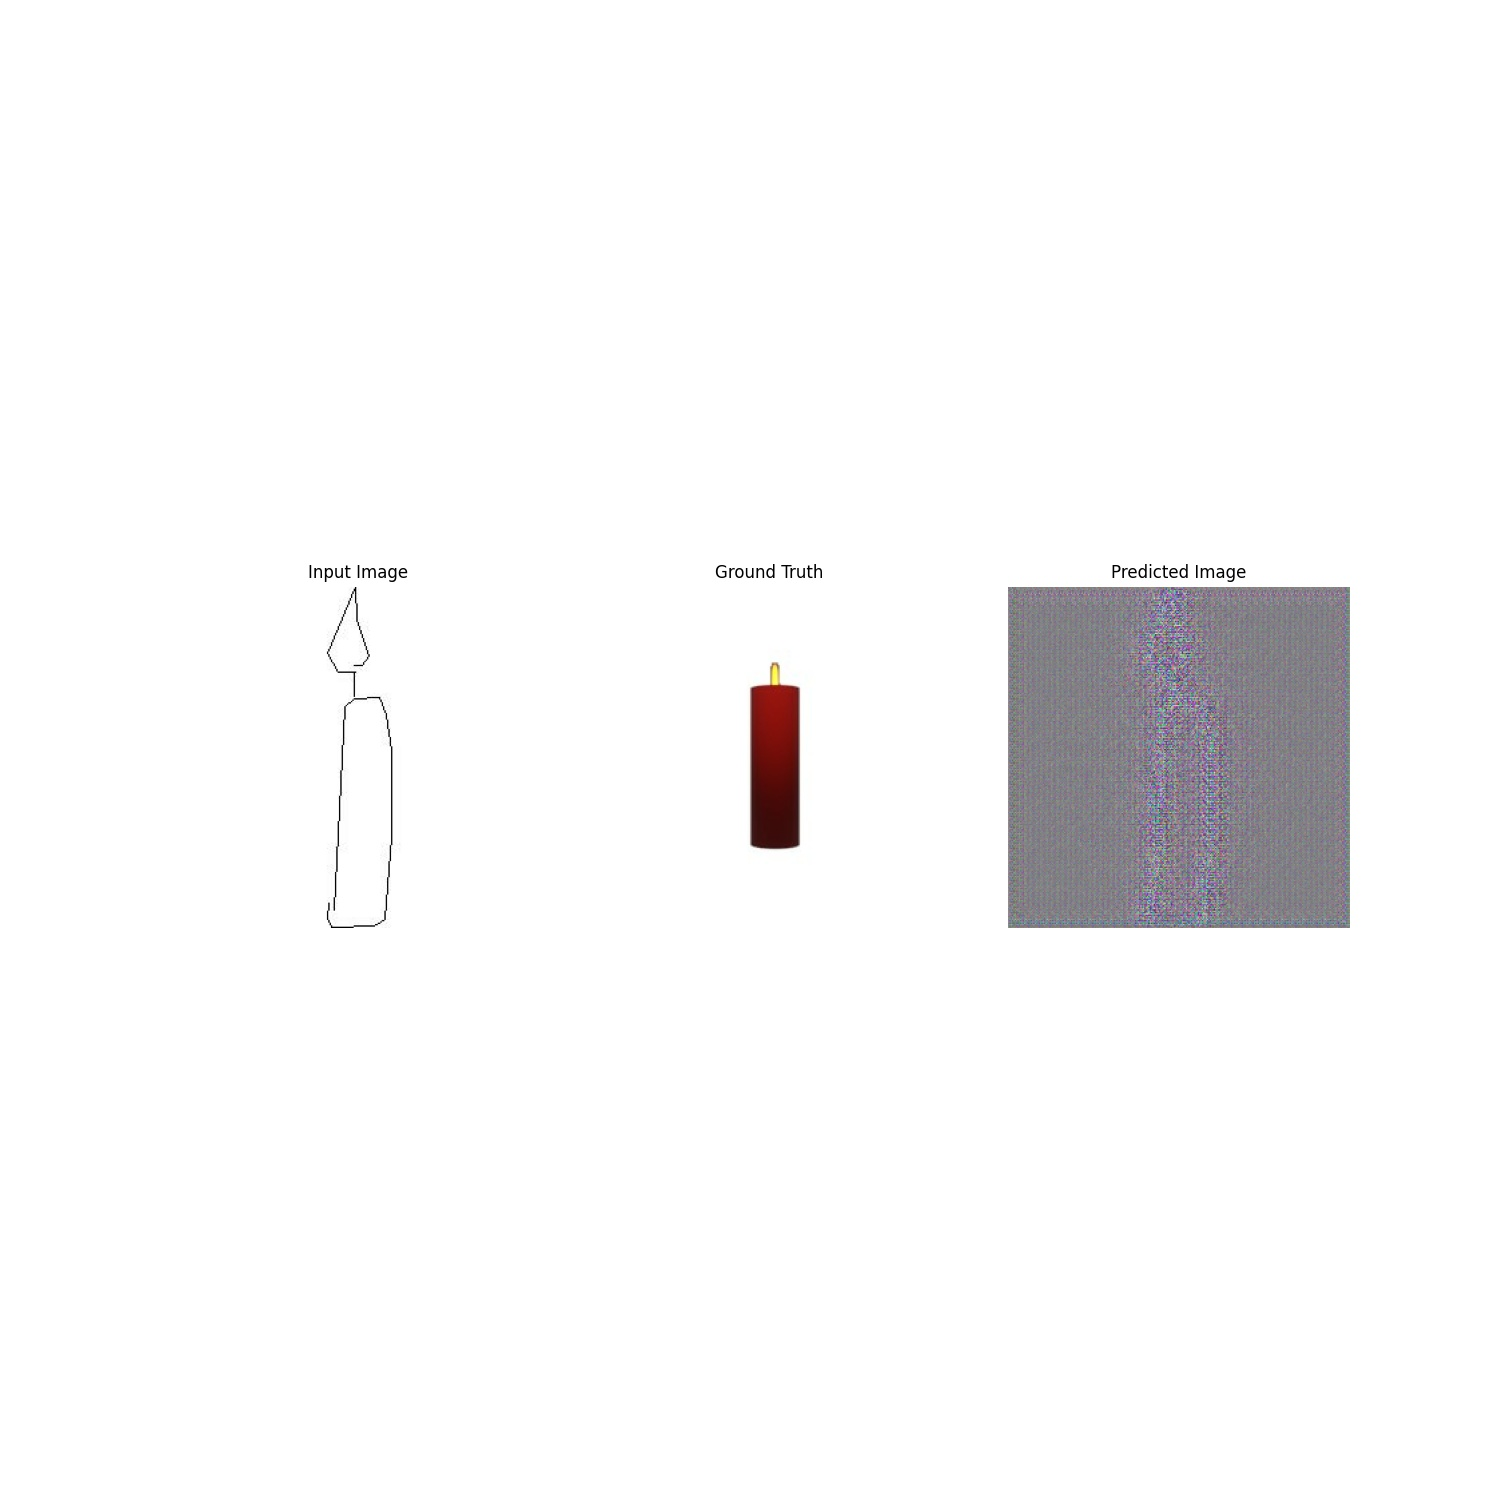
\includegraphics[width=0.3\textwidth]{bilder/0.jpg}
	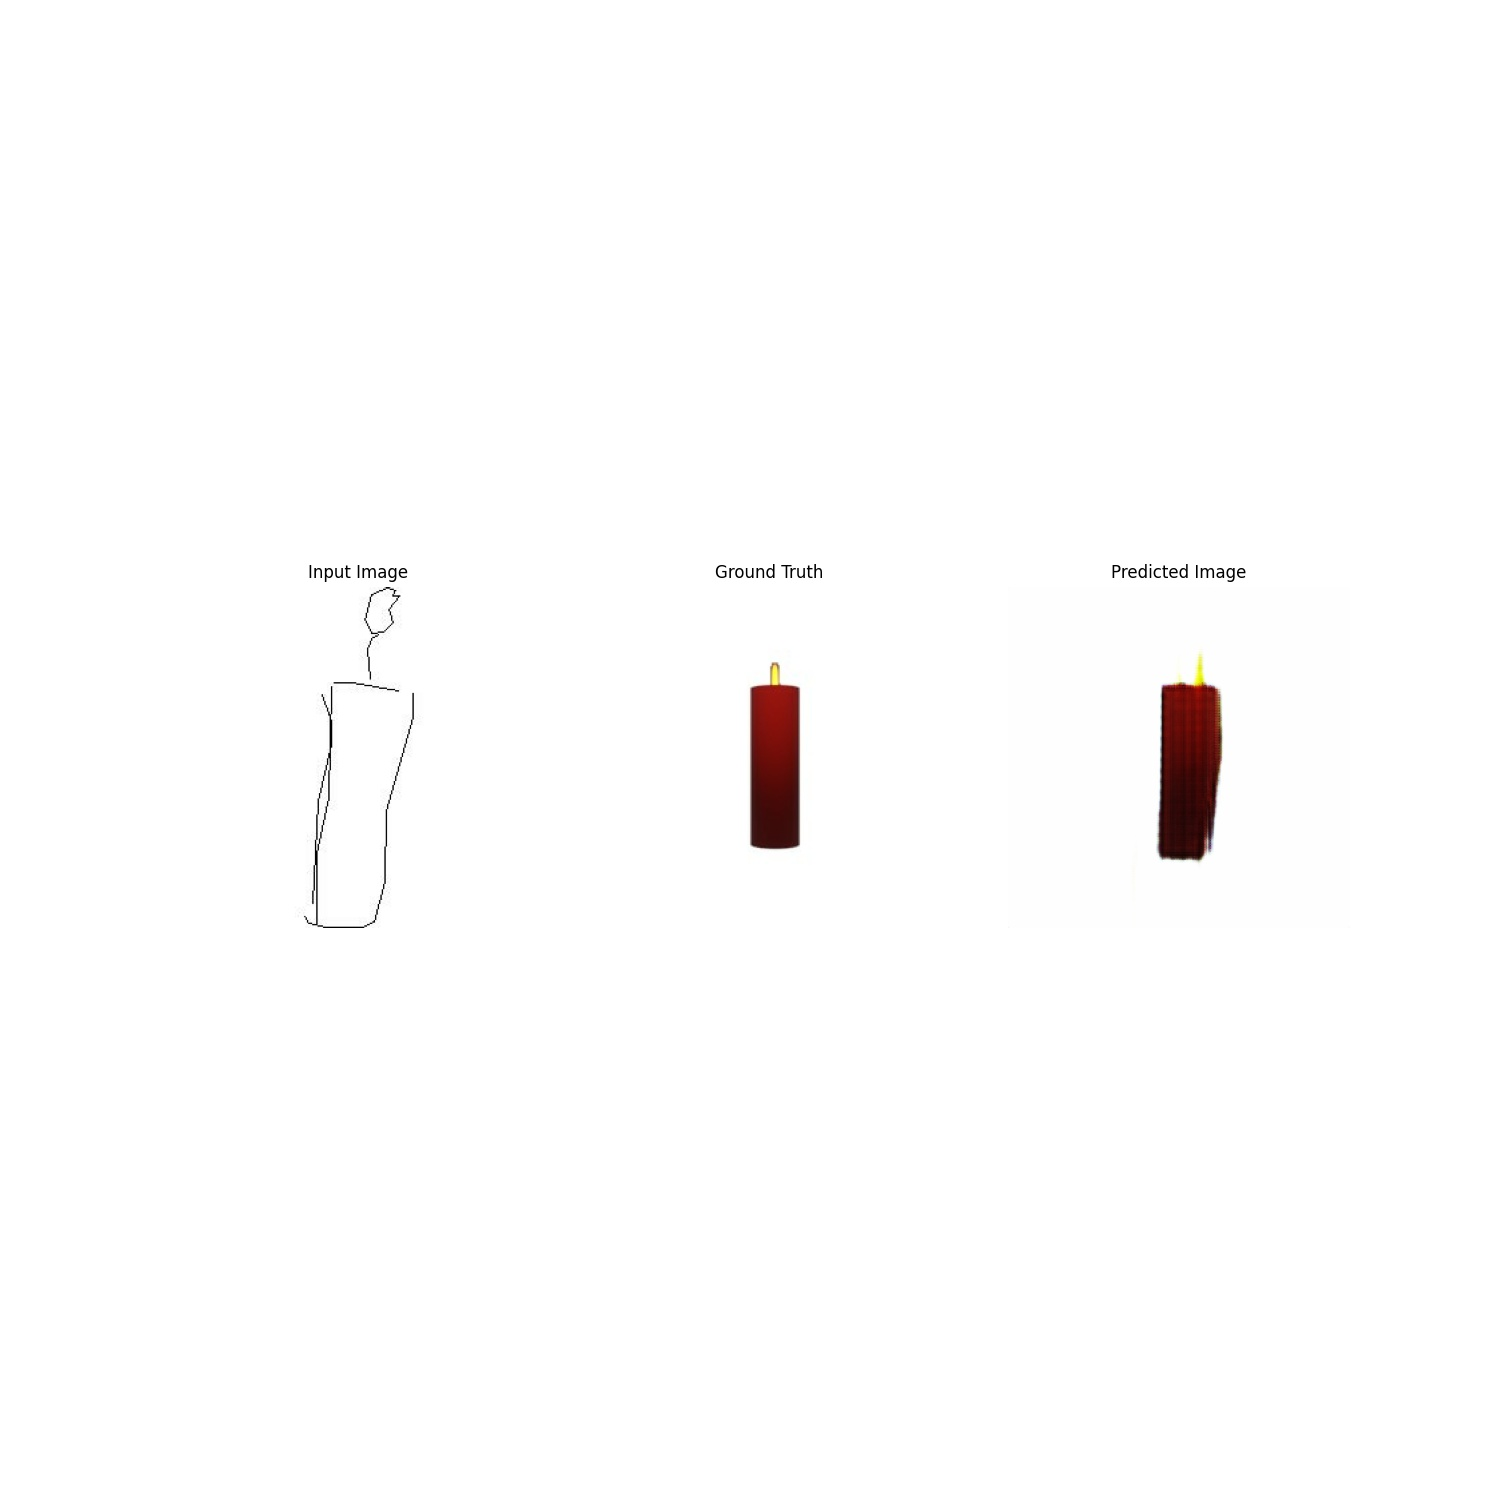
\includegraphics[width=0.3\textwidth]{bilder/1.jpg}
	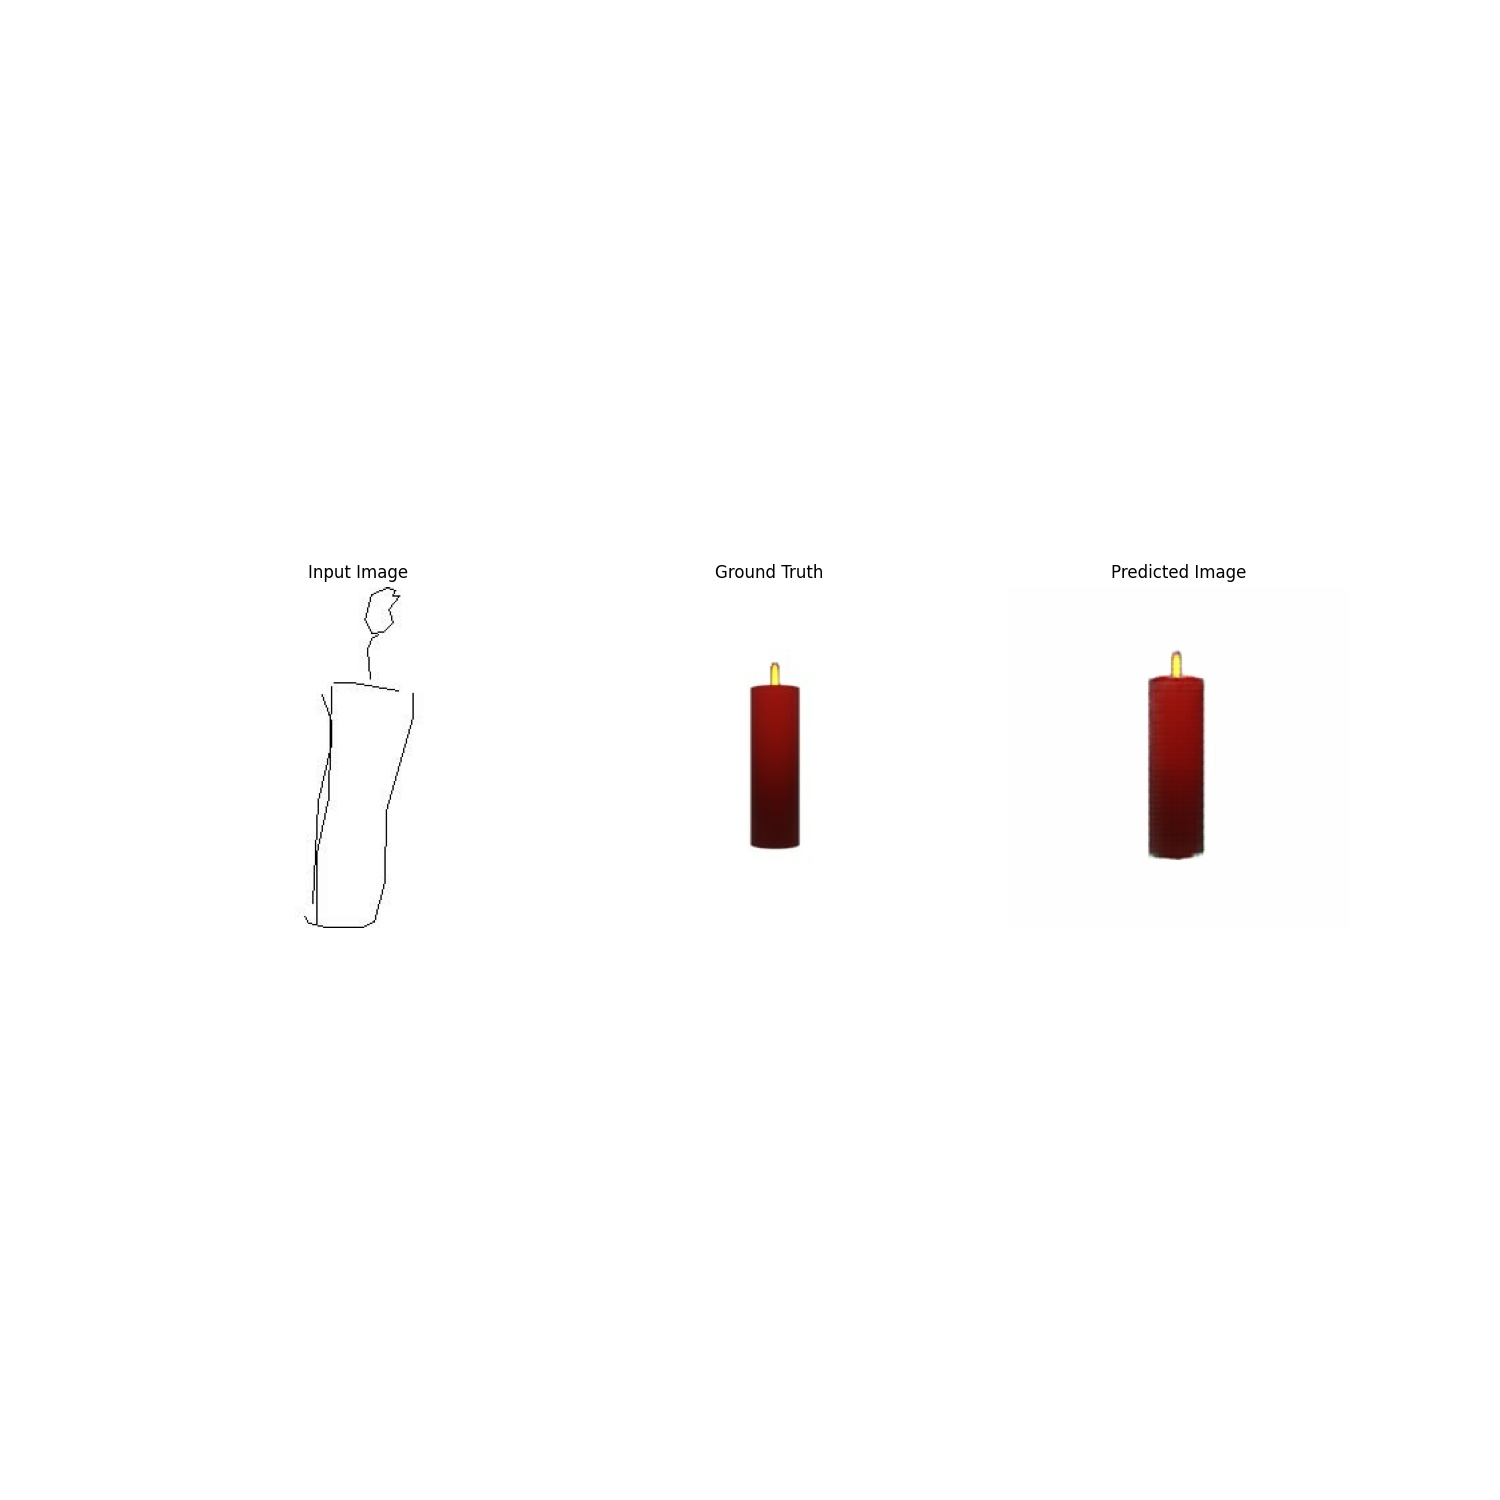
\includegraphics[width=0.3\textwidth]{bilder/15.jpg}
	\caption[Verschiedene Trainingsschritte]{Das Modell generiert das Ergebnis schrittweise aus zufälligem Rauschen. Nach 15000 Trainingsschritten ist das Ergebnis zufriedenstellend.}
	\label{fig:trichter}
\end{figure}

% Die Arbeit verfolgt das Ziel, verschiedene bewährte Architekturen künstlicher
% neuronaler Netze zur Generierung von Bildern zu untersuchen und in einem
% praxisorientierten Zusammenhang zu testen. Ich zeige mehrere Möglichkeiten,
% wirklichkeitsnahe Bilder von Alltagsgegenständen aus Skizzen, die durch Benutzer
% erstellt wurden, mittels eines künstlichen neuronalen Netzes zu generieren. Die
% Bilddateien der Skizzen sowie die generierten Bilddateien können dabei aus
% RBG-Pixelinformationen bestehen oder die Grafik mittels Bildkoordinaten beschreiben,
% wie es bei Vektorgrafiken und 3D-Modellen der Fall ist. Eine Anwendung der
% Ergebnisse ist beispielsweise als Feature eines Grafiktablets oder eines
% Smartboards denkbar.

\section{Bisherige Arbeiten}
\label{sec:related}
Künstliche neuronale Netze finden erst seit wenigen Jahren breite Aufmerksamkeit,
seit auch Heimcomputer in der Lage sind die hohe Anzahl der erforderlichen
Rechenoperationen in annehmbarer Zeit auszuführen. Seitdem sind wenige,
englischsprachige Einführungen in die Thematik entstanden. Ein häufig genanntes
Buch ist ``Deep Learning'', das online kostenfrei zugänglich ist \cite{Goodfellow-et-al-2016}.
Ebenfalls online kostenfrei ist das Buch ``Dive into Deep Learning'' \cite{zhang2020dive}.
Ein weiteres, praxisorientierteres Buch ist ``Deep Learning with Python'' \cite{chollet2021deep}, dessen
zweite Auflage bald herausgegeben wird.

Erste Recherchen haben verschiedene Arten und Implementierungen Bilder generierender künstlicher neuronaler Netze herausgestellt. Das Model aus ``DRAW: A Recurrent Neural Network For Image Generation'' \cite{gregor2015draw} kann darauf trainiert werden, handschriftliche Ziffern wie die des MNIST-Datasets zu generieren.

Die Schlüsselerkenntnis in ``A Neural Algorithm of Artistic Style'' \cite{gatys2015nst} ist, dass Inhalt und Stil eines Bildes voneinander getrennt werden können. Das Model kann zum Beispiel den Stil eines Künstlers auf das Bild eines anderen übertragen.

In anderen Ansätzen mit rekurrenten neuronalen Netzen wird jedes Eingabebild in eine Sequenz von Pixeln umgeformt. Anschließend wird das künstliche neuronale Netz darauf trainiert, teilweise geschwärzte Bilder wieder zu vervollständigen \cite{chen2020generative}, \cite{oord2016pixel}. Es werden auch Bilder generiert und die Fähigkeit des jeweiligen Models, die Darstellung von Bildern zu lernen, untersucht und mit der anderer Models verglichen. Ein weiterer, ebenfalls rekurrenter Algorithmus generiert Bilder aus textuellen Beschreibungen \cite{ramesh2021zeroshot}.

Besondere Aufmerksamkeit habe ich den Generative Adversarial Networks \cite{goodfellow2014generative} gegeben. Die Ergebnisse dieser Familie von künstlichen neuronalen Netzen sind teilweise erstaunlich gut, und es gibt bereits einige Beispielanwendungen und frei verfügbaren Quelltext. Je nach Anwendung des Models variiert die Qualität der Resultate.

Die vielseitigste Generierung von Bildern bietet Image-To-Image-Translation with Conditional Adversarial Networks \cite{isola2018imagetoimage}. In der Arbeit werden Labels in Fotos zurückübersetzt, Schwarzweißbilder coloriert und weitere Anwendungsbeispiele gezeigt. Vor allem die Übersetzung ``Kanten nach Foto'' (``Edges to Photo'') ist für mein Vorhaben relevant. Das Dokument enthält dafür mehrere Beispiele und Hinweise für die Anpassung der Hyperparameter. Der Algorithmus setzt auf Generative Adversarial Networks \cite{goodfellow2014generative} und Conditional Generative Adversarial Networks \cite{mirza2014conditional} auf.

In ``Unsupervised Representation Learning with Deep Convolutional Generative Adversarial Networks'' \cite{radford2016unsupervised} werden ebenfalls
realitätsnahe Ergebnisse erzielt. Anders als bei den bisher erwähnten Arbeiten
wird Unsupervised Learning verwendet, um das künstliche neuronale Netz zu trainieren.

\begin{figure}[h]
	\centering
	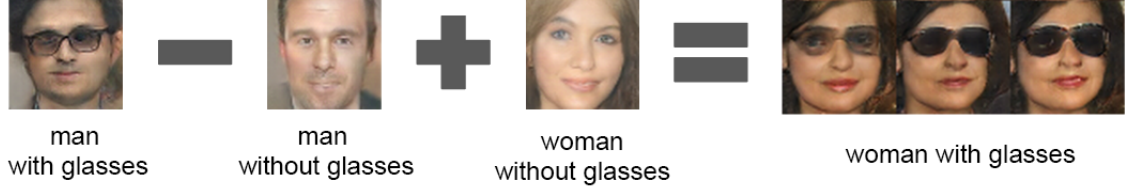
\includegraphics[width=1.0\textwidth]{bilder/image_arithmetic.png}
	\caption[Bildarithmetik]{Bildquelle: ``Unsupervised Representation Learning with Deep Convolutional Generative Adversarial Networks'' \cite{radford2016unsupervised} \newline Unter anderem werden dort Bilder in einer Art Arithmetik miteinander kombiniert, um ein neues Ergebnis zu erzeugen.}
	\label{fig:unsupervisedexamples}
\end{figure}

\begin{figure}[h]
	\centering
	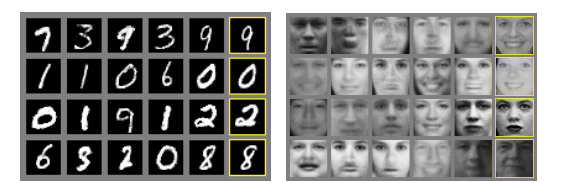
\includegraphics[width=1.0\textwidth]{bilder/mnist_faces.png}
	\caption[GAN Beispielbilder]{Bildquelle: ``Generative Adversarial Nets'' \cite{goodfellow2014generative} \newline Dieses Dokument zeigt mehrere Beispiele generierter Bilder. Es ist deutlich zu erkennen, wie gut der Algorithmus geeignet ist Bilder zu generieren. Die gelb gerahmten Bilder sind die Ground Truth aus dem jeweiligen Trainingsset.}
	\label{fig:ganexamples}
\end{figure}

\pagebreak

\begin{figure}[h]
	\centering
	\imagetranslation{bilder/edges2cats_a}{bilder/edges2cats_b}
	\hspace{.5cm}
	\imagetranslation{bilder/fotogenerator_a}{bilder/fotogenerator_b}
	\hspace{.5cm}
	\imagetranslation{bilder/sketch2portrait_a}{bilder/sketch2portrait_b}
	\label{fig:pix2pixexamples_1}
\end{figure}

\begin{figure}[h]
	\centering
	\imagetranslation{bilder/pokemon_a}{bilder/pokemon_b}
	\hspace{.5cm}
	\imagetranslation{bilder/shoe_a}{bilder/shoe_b}
	\hspace{.5cm}
	\imagetranslation{bilder/handbag_a}{bilder/handbag_b}
	\caption[Bildarithmetik]{Bildquelle: ``Image-To-Image-Translation with Conditional Adversarial Networks'' \cite{isola2018imagetoimage} \newline In dem Paper zu Pix2Pix sind viele Beispiele für die Generierung von Bildern aus Handzeichnungen oder Ergebnissen einer Kantenerkennung (zum Beispiel Canny Edge Detection) enthalten.}
	\label{fig:pix2pixexamples_2}
\end{figure}

\begin{figure}[h]
	\centering
	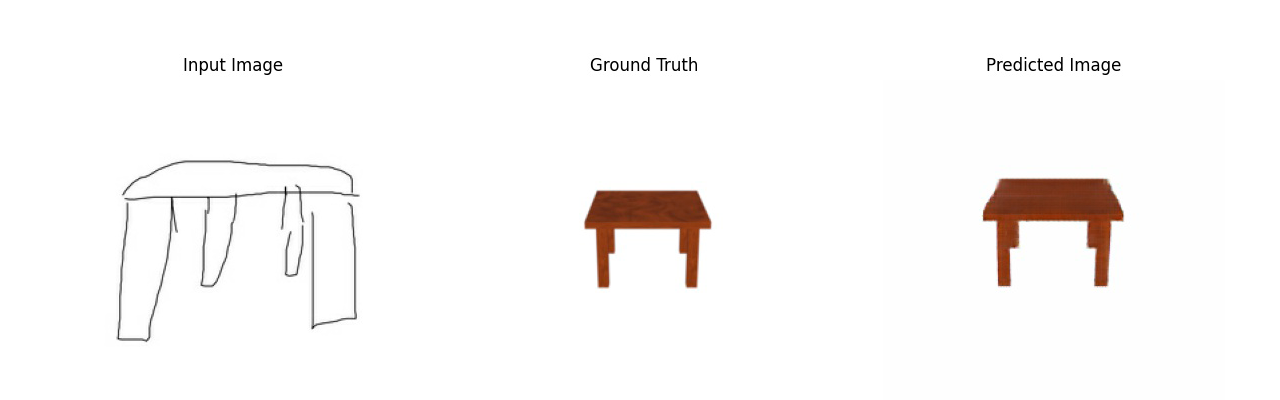
\includegraphics[width=0.6\textwidth]{bilder/table1small.png}
	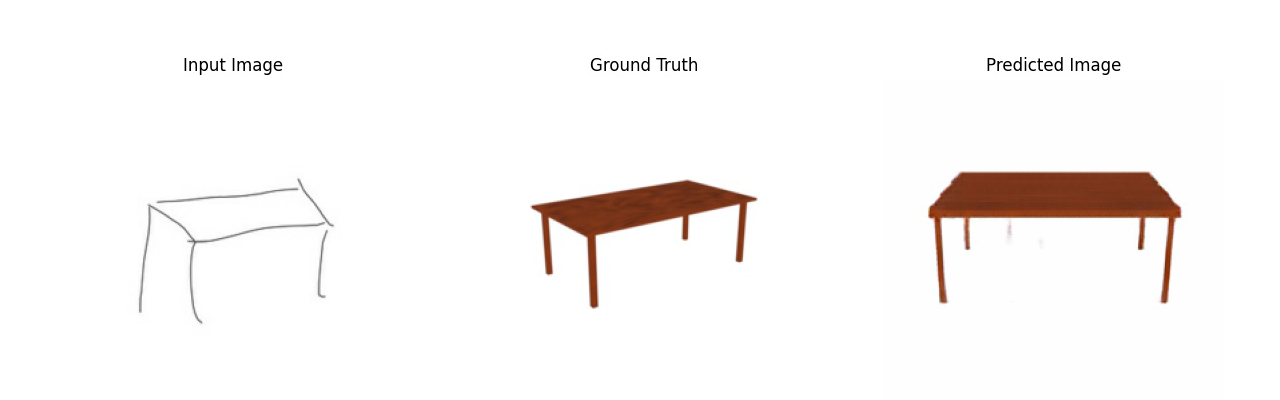
\includegraphics[width=0.6\textwidth]{bilder/table2small.png}
	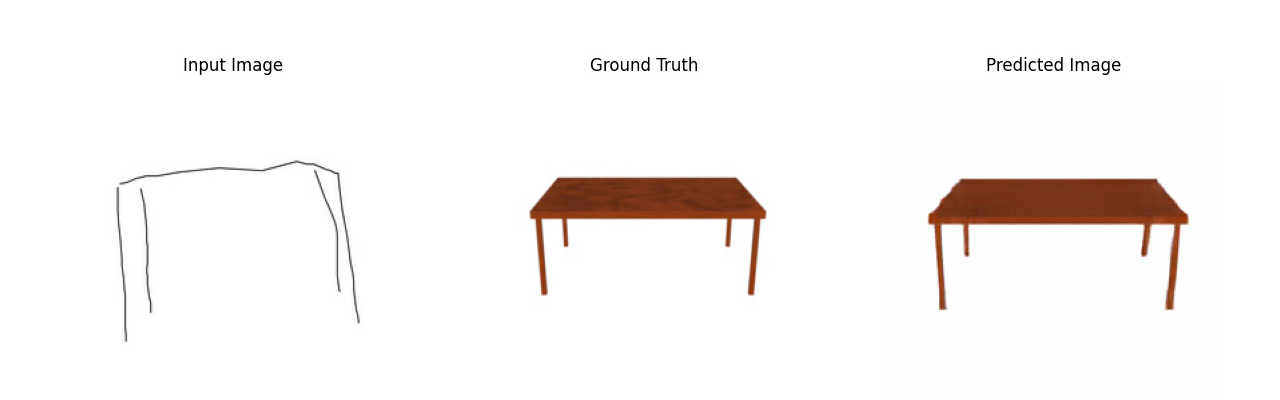
\includegraphics[width=0.6\textwidth]{bilder/table3small.png}

	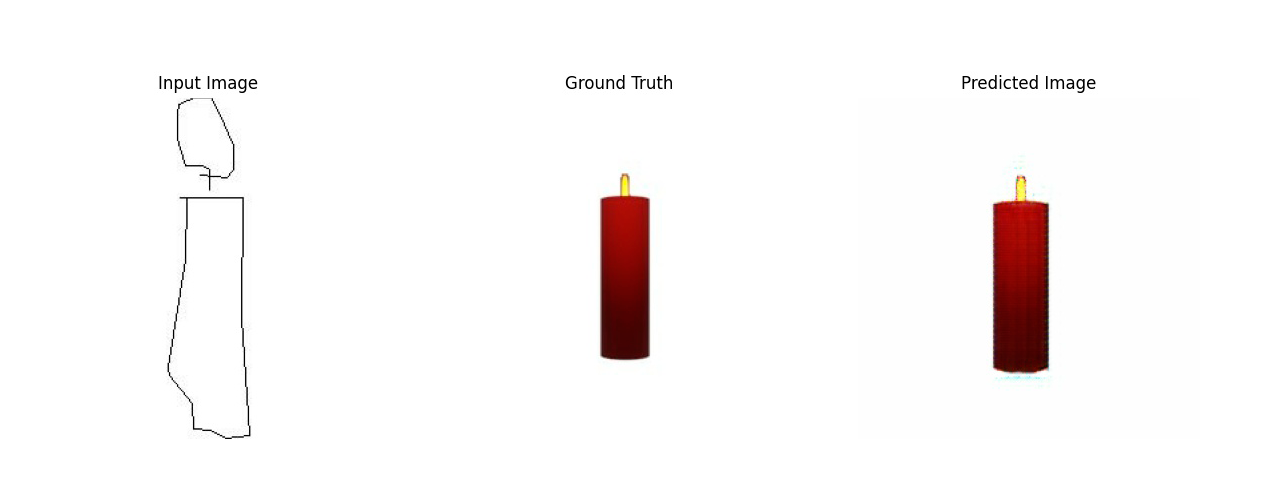
\includegraphics[width=0.6\textwidth]{bilder/candle1small.png}
	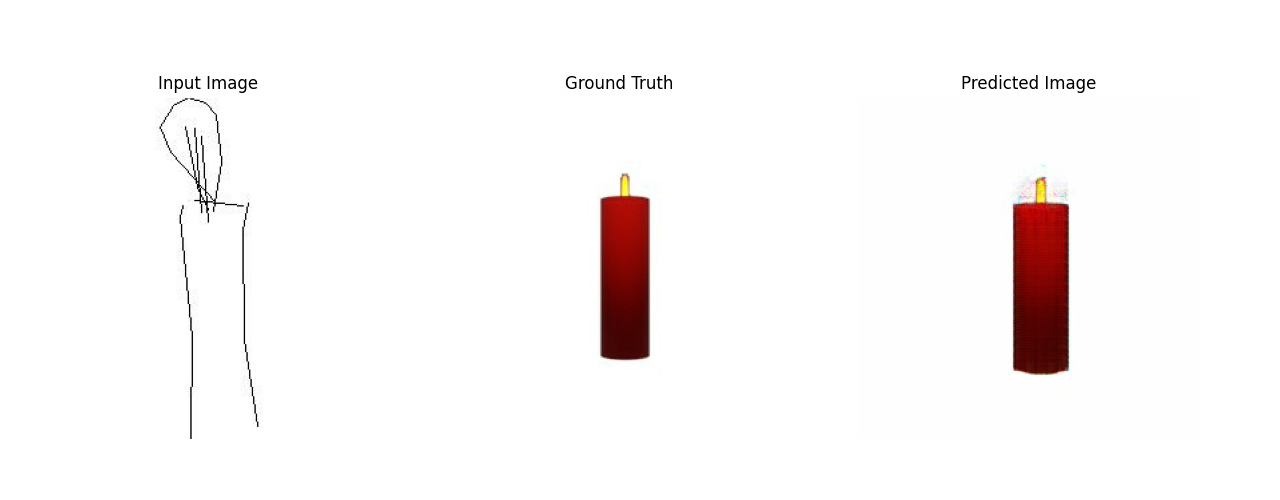
\includegraphics[width=0.6\textwidth]{bilder/candle2small.png}
	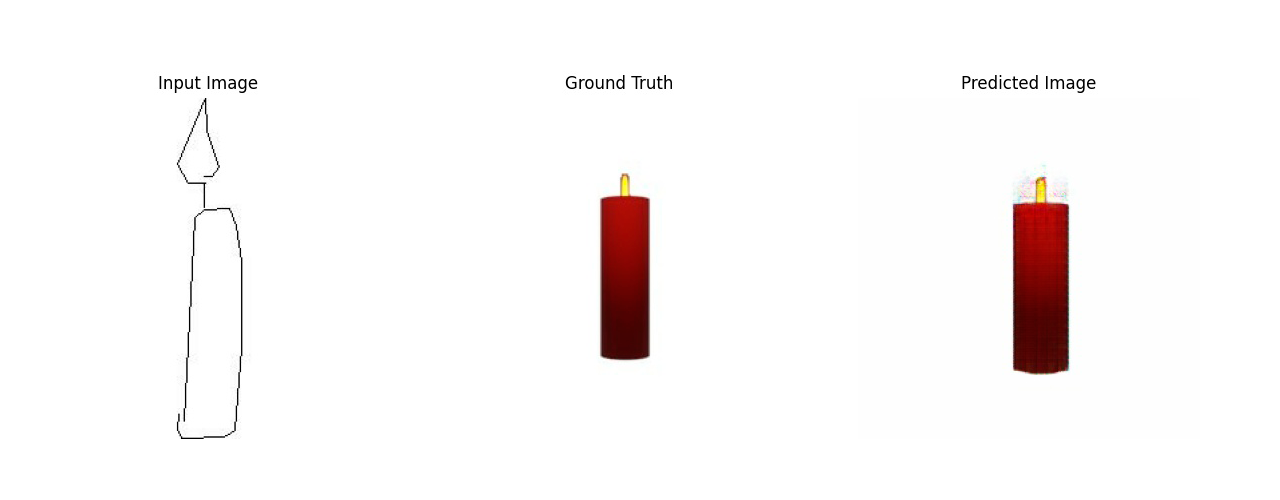
\includegraphics[width=0.6\textwidth]{bilder/candle3small.png}
	\caption[Eigene Beispiele]{Meine Ergebnisse zeigen, dass aus einer Handzeichnung ein fotorealistisches Bild generiert werden kann. Die generierten Bilder nehmen ungefähr die Proportionen der Handzeichnungen an, erstellen realistische Darstellungen der Gegengenstände und fügen Texturen und Lichteffekte hinzu.}
	\label{fig:myexamples}
\end{figure}

Blender ist ein 3D-Computergrafikprogramm mit Werkzeugen für die Modellierung und Animation von Objekten und Charakteren und zur Erstellung von Hintergrundszenen. Szenen können als Standbilder hergestellt werden. Animierte Sequenzen können für Videoproduktionen genutzt werden. Modelle und Szenen werden durch Farben und Texturen noch aufgewertet, wodurch brillante realistische Effekte produziert werden. Die Standbilder und Videos können als Kunstwerke oder als architektonisch oder wissenschaftliche Präsentationen Anwendung finden. \cite{blain2020blender}


\cleardoublepage
\chapter{Modell}
\label{ch:model}

\section{Tensoren}
Mehrdimensionale Arrays, in NumPy ndarray (N-Dimensional Array) genannt, werden auch Tensoren genannt. Gennerell verwenden alle derzeitigen Systeme für Maschinelles Lernen Tensoren als zugrundeliegende Datenstruktur. Tensoren sind elementar für dieses Fachgebiet. \cite{chollet2017dlpython}

In seinem Kern ist ein Tensor ein Container für numerische Daten. Tensoren sind die Verallgemeinerung der Matrizen für eine beliebige Anzahl Dimensionen. Im Zusammenhang mit Tensoren werden die Dimensionen häufig Achsen gennannt. Die Anzahl der Achsen wird auch als Stufe bezeichnet. Ein Skalar ist ein Tensor nullter Stufe. Ein Vektor ist ein Tensor erster Stufe und eine Matrix ein Tensor zweiter Stufe. \cite{chollet201chollet2017dlpython7}

Der Begriff der Dimension, der für Vektoren und Matrizen eindeutig ist, wird für Tensoren in der Literatur unterschiedlich verwendet.  \cite{chollet2017dlpython} In dieser Arbeit soll die Dimension einer Achse eines Tensors die Anzahl der numerischen Werte entlang dieser Achse bezeichnen.

Bilder erscheinen als Tensoren dritter Stufe, deren Achsen der Höhe, Breite und den Farbkanälen (Rot, Grün und Blau) entsprechen. \cite{zhang2020dive}

Ein Tensor ist durch drei Schlüsselattribute definiert:
\begin{itemize}
\item Anzahl der Achsen (Stufe): Zum Beispiel hat ein Tensor dritter Stufe drei Achsen, und eine Matrix hat zwei Achsen. In Python-Bibliotheken wie NumPy oder Tensorflow wird sie auch als $ndim$ des Tensors bezeichnet.
\item Form: Dies ist ein Tupel aus Ganzzahlen, das die Dimension jeder Achse beschreibt. Beispiele sind $(3, 5)$ für die Form einer Matrix und $(3, 3, 5)$ für einen Tensor dritter Stufe. Ein Vektor hat eine Form mit einem einzelnen Element, etwa so: $(5,)$, während ein Skalar eine leere Form hat: $()$.
\item Datentyp (in Python-Bibliotheken gewöhnlich $dtype$ genannt): Dies ist der Typ der im Tensor enthaltenen Daten. Zum Beispiel könnte der Datentyp eines Tensors $float16$, $float32$, $float64$, $uint8$ und so weiter sein.
\end{itemize}
\cite{chollet2017dlpython}

Viele in dieser Arbeit verwendeten Tensoren beschreiben RBG-Bilddaten. Sie sind deshalb dritter Stufe, und die enthaltenen Daten sind Ganzzahlen zwischen $0$ und $255$. Die Form der durch das künstliche neuronale Netz generierten Bilder ist $(256, 256, 3)$. Die Dimensionen beschreiben hier also die Breite, Höhe und Farbtiefe der Bilddateien.


\section{Logistische Regression}
\label{sec:logreg}
Ein vergleichsweise einfacher Algorithmus des Maschinellen Lernens ist Logistic Regression oder Softmax Regression. Es lassen sich damit Klassifizierungen durchführen. Bei binären Klassifizierungen werden die Eingaben in zwei Kategorien unterteilt. Häufige Beispiele sind fehlerfreie oder fehlerhafte Produktionsergebnisse, ärztliche Befunde einer bestimmten Krankheit oder Gesundheit und ob in einem Bild ein bestimmtes Objekt vorhanden ist oder nicht.

Bei der Multiclass Logistic Regression werden die Eingaben in mehr als zwei Klassen unterteilt. Es lassen sich damit beispielsweise in einem Bild  verschiedene Arten von Fahrzeugen, Gegenständen oder Tieren unterteilen.

Diagramm: Ein-Schicht-NN (Die Ausgabeschicht wird nicht mitgezählt) Logistic Regeression kann mit einer einzelnen oder mehreren neuronalen Schichten imlementiert sein. Das künstliche neuronale Netz in Abb. x besitzt eine einzelne aus drei Einheiten bestehende Schicht. Eine Einheit besteht zunächst aus einer differenzierbaren Funktion. Oft ist das eine Multiplikation der Eingaben $X$ mit einer Anzahl lernbaren Parametern $W$ und eine anschließende Addition mit Bias-Werten $b$. Die Ausgabe einer Schicht wird oft mit $\hat{y}$ bezeichnet:
\begin{align}
\hat{y} = WX+b
\end{align}

Dieser folgt eine Aktivierungsfunktion, die dem errechneten Wert einen anderen Wert zuordnet, der entweder nahe $0$ oder nahe $1$ liegt (gelegentlich nahe $-1$ oder nahe $1$). Beispiele für Aktivierungsfunktionen sind Sigmoid:
\begin{align}
sig(t) = \frac{1}{1+e^{-t}}
\end{align}

und Rectified Linear Unit, kurz ReLU:
\begin{align}
f(x) = max(0, x)
\end{align}

oder auch Leaky ReLU:
\begin{align}
f(x) = max(0.01x, x)
\end{align}

In einigen künstlichen neuronalen Netzen werden zusätzlich die Eingaben für jede Schicht normalisiert, wodurch die Minimierung der Verlustfunktion (Gradient Descent) optimiert werden kann.

\section{Deep Neural Networks}
\label{sec:dnn}

\section{Convolutional Neural Networks}
\label{sec:cnn}
Für Bilddaten wendet ein CNN diese Operation typischerweise auf zwei dreidimensionale Matrizen an, nämlich einerseits auf die Eingabedaten und andererseits auf einen sogenannten Filter oder auch Kernel. Die Eingabedaten sind in der ersten Schicht des Netzes die RGB-Pixelinformationen und in allen weiteren konvolutionalen Schichten die Ausgabe der vorherigen Schicht. Ein Filter ist eine Anzahl von trainierbaren Parametern, in diesem Fall auch eine . Beide Matrizen haben also die Form $(H\ x\ W\ x\ C)$, wobei $H$ die Höhe, $W$ die Breite und $C$ die RGB-Farbwerte repräsentiert.

Jede der drei Matrixdimensionen variiert üblicherweise zwischen den verschiedenen Schichten des Netzes. In fast allen CNNs (\cite{Goodfellow-et-al-2016}, \cite{Lecun99objectrecognition}, \cite{RFB15a}, \cite{isola2018imagetoimage}) nimmt die Kardinalität zunächst ab. Die Reduktion kann durch die Konvolution selbst entstehen oder durch Pooling-Schichten. Beim Pooling werden aus benachbarten Matrixkoeffizienten meist das Maximum, seltener der Durchschnitt oder andere Aggregierungen gebildet. Auf diese Weise wird das neuronale Netz darauf trainiert die relevanten Informationen zu extrahieren. \cite{Goodfellow-et-al-2016}

Den konvolutionalen Schichten folgt in einigen Anwendungsfällen eine voll vernetzte Schicht (engl. Fully Connected Layer, FC), in der für jedes Neuron mit jedem Neuron der vorherigen Schicht eine Verbindung besteht. Besonders für die Bilderkennung ist diese Architektur gut geeignet. Die Ausgabe des neuronalen Netzes ist dann ein Vektor, beispielsweise von Wahrscheinlichkeitswerten für das Vorhandensein bestimmter Objekte und gegebenenfalls Bildkoordinaten der erkannten Objekte. Im Fall der Bildgenerierung ist die Ausgabe aber wieder eine Matrix von RGB-Pixelinformationen in der Form $(H\ x\ W\ x\ 3)$.

\section{U-Net-Architektur}
\label{sec:unet}
Die bis hierhin beschriebenen neuronalen Netze besitzen eine gradlinige Struktur, in der die Ausgabe einer Schicht nur an die nächste Schicht übergeben wird. Bei zunehmender Anzahl der Schichten verbessert sich die Performance neuronaler Netze mit diesem Aufbau zunächst, aber verschlechtert sich bei zu vielen Schichten wieder. In einem Residual Neural Network (ResNet) verhindern zusätzliche Verbindungen zwischen nicht direkt aufeinanderfolgenden Schichten diesen Performanceverlust.

Ein U-Net ist eine spezielle Form eines ResNets. Es hat eine annähernd symmetrische Struktur, in der sich die Kardinalitäten der Matrizen zuerst verringern und anschließend wieder erhöhen. U-Nets erzielen selbst mit wenigen Trainingsdaten gute Ergebnisse und benötigen dafür vergleichsweise wenig Rechenleistung. \cite{he2015deep}

\section{Generative Adversarial Networks}
\label{gan}
Ein Generative Adversarial Network (GAN)besteht zunächst aus einem Generator und einem Discriminator \cite{goodfellow2014generative}. Der Generator lernt während des
Trainings täuschend echt aussehende Bilddaten zu generieren. Der Discriminator
wird dagegen darauf trainiert, echte von generierte Bildern zu unterscheiden.
Anschließend können beide Modelle ``gegeneinander antreten''. Deswegen wird es
Generative \textit{Adversarial} Network genannt.

GANs unterscheiden sich von anderen Modellen durch ihren Aufbau und in Bezug auf das Trainingsziel. Künstliche neuronale Netze ermitteln häufig einen skalaren Wert wie beispielsweise einen Wahrscheinlichkeitswert und minimieren zu diesem Zweck eine Verlustfunktion. In einem GAN sind zwei CNNs im Einsatz. Das erste, der Generator, erstellt Tensoren n-ter Klasse. In diesem Beispiel sind das RGB-Bildinformationen. Das zweite CNN wird Discriminator genannt und bekommt als Eingabe die Ausgabe des ersten CNNs. Der Discriminator wird darauf trainiert, generierte Bilder von Bildern aus dem Trainingsset zu unterscheiden. Er minimiert also eine Verlustfunktion. Der Generator wird darauf trainiert, diese Verlustfunktion zu maximieren. Dieser Vorgang stammt aus der Spieltheorie und heißt Minimax. \cite{goodfellow2014generative}

Eine Erweiterung des GANs ist das Conditional Generative Adversarial Net (cGAN). In cGANs erhält der Generator zusätzliche Eingabedaten ($y$, ``Ground Truth''), die Hinweise für die Generierung enthalten. Der Discriminator erhält diese zusätzlichen Daten ebenfalls, um die Erkennung während des Trainings zu optimieren. \cite{mirza2014conditional}

\section{Image-To-Image-Translation}
\label{sec:pix2pix}
Der Image-To-Image-Translation-Algorithmus oder kurz Pix2Pix-Algorithmus verwendet ein GAN, um Bilder in Bilder zu übersetzen. Dafür kommen zwei CNNs zum Einsatz, nämlich eins für den Generator und eins für den Discriminator. \cite{isola2018imagetoimage}

Die Datei \hyperref[pix2pixpy]{main.py} befindet sich im Anhang und ist die Implementierung, die für diese Arbeit hauptsächlich verwendet wurde.

Die erste Funktion namens \lstinline|load| öffnet eine Datei und liest diese als JPEG-Bilddatei. Sie wird verwendet, um die Trainingsdaten zu laden. Weil die Trainingsdaten aus zwei Bildern pro Datei bestehen, nämlich jeweils einem Eingabebild und dem erwarteten Ergebnis (Ground Truth), extrahiert die Funktion zusätzlich die beiden Bilder und gibt jede in einer eigenen Variablen zurück.

Die Funktion \lstinline|resize| ist ebenfalls für die Verarbeitung zweier Bilder vorgesehen und skaliert beide auf die übergebene Breite und Höhe.

Die Funktion \lstinline|random_crop| stellt einen zufälligen Ausschnitt der zwei Eingabebilder frei. Sie wird aufgerufen, nachdem die Eingabebilder hochskaliert wurden. In der Referenzimplementierung wie auch in dieser Arbeit beträgt die Bildgröße vorher $286x286$ Pixel und $256x256$ Pixel nach dem Freistellen. Die zurückgegebenen Bilder haben dann wieder die gleichen Abmessungen wie die Eingabedaten.

In der Funktion \lstinline|normalize| werden die RGB-Werte der beiden Eingabebilder normalisiert. Dadurch sollen zu große Schritte auf dem Gradienten verhindert werden, die das Konvergieren verhindern könnten. \cite{chollet2017dlpython} Die RGB-Werte sind zunächst als Ganzzahlen im Bereich von 0 bis 255 gegeben und werden in Fließkommazahlen im Bereich -1 bis 1 umgerechnet.

In \lstinline|random_jitter| wird zunächst \lstinline|resize| aufgerufen, um die Eingabebilder auf 286x286 Pixel zu skalieren. Anschließend wird \lstinline|random_crop| auf die skalierten Bilder angewendet. Schließlich werden aufgrund einer Zufallszahl beide Eingabebilder mit einer Wahrscheinlichkeit von 50 Prozent gespiegelt.

Die beiden Funktionen \lstinline|load_image_train| und \lstinline|load_image_test| laden die Eingabe- und Referenzbilder (Ground Truth), skalieren diese auf 256x256 Pixel und normalisieren die Eingabedaten durch Aufrufe der Funktionen \lstinline|load|, \lstinline|resize| und \lstinline|normalize|. Nur die Funktion zum Laden der Trainingsbilder ruft für die geladenen Bilder \lstinline|random_jitter| auf.

Die Funktion \lstinline|downsample| erzeugt eine Schicht eines CNNs mit optionaler Batch Normalization und der Leaky-ReLU-Aktivierungsfunktion. Diese Schichten werden im Encoder des Generators sowie im Discriminator verwendet. Batch Normalization kommt nur in der jeweils ersten Schicht des Generators und des Diskriminators nicht zum Einsatz.

In der Funktion \lstinline|upsample| entstehen die übrigen CNN-Schichten des Generators. Der Entfaltung, bei der die Faltung der Funktion \lstinline|downsample| umgekehrt wird (engl. Transposed Convolution \cite{zaccone2018tensorflow}), folgt hier immer die Batch Normalization sowie optional Dropout mit einem Wahrscheinlichkeitswert von $0.5$. Das ist in den ersten drei Schichten des Decoders im Generator der Fall und bedeutet, dass statistisch die Hälfte der Aktivierungen „fallengelassen“ werden, also nicht in das Trainingsergebnis eingehen. Als Aktivierungsfunktion kommt ReLU zum Einsatz.

In \lstinline|build_generator| werden die Schichten des Generators zusammengefügt. Im Encoder wird acht Mal \lstinline|downsample| aufgerufen, bis die Dimensionen des Eingabetensors, die am Anfang der Bildgröße entsprechen (Breite und Höhe, also $256x256$ Pixel), durch die Konvolution auf $1$ reduziert sind. Die Dimension, welche die Anzahl Farbkanäle der Eingabebilder repräsentiert, erhöht sich im Encoder auf den Wert $512$. Die Werte dieser Achse werden als Features \cite{zhang2020dive} \cite{chollet2017dlpython} \cite{zaccone2018tensorflow} bezeichnet.

Der Decoder ruft seinerseits sieben Mal \lstinline|upsample| auf und führt eine weitere Entfaltung durch, wodurch die Dimensionen des bearbeiteten Tensors wieder jeweils dieselbe Form wie in den Eingabebildern annehmen. Schließlich werden die Skip-Connections zwischen den Schichten 1 bis 8 des Encoders und des Decoders hergestellt.

In der Funktion \lstinline|generator_loss| ist die Backpropagation des Generators implementiert. Zuerst wird dafür die Kreuzentropie des Ergebnisses des Discriminators und eines gleich großen Tensors, der mit Einsen initialisiert wird, gebildet. TODO: crossentropy Das Ergebnis ist das GAN-Loss. Anschließend kommt die L1 Loss Function, auch Mean Absolute Error genannt, zum Einsatz:
\begin{align}
  \mathcal{L} _{L1}(G) = \mathbb{E}_{x,y,z}[\|y - G(x,z)\|_1]
\end{align}
wobei $x$ für die Eingabebilder, $y$ für die Ground Truth und $z$ für das Ergebnis des des Generators, also das generierte Bild, steht \cite{isola2018imagetoimage}. Dieses L1-Loss wird aus dem Durchschnitt der absoluten Differenz der Ground Truth und des Generatorergebnisses berechnet. Der Gesamtverlust des Generators ist das GAN-Loss plus das Produkt aus dem Regularisierungsparameter Lambda, der konstant $100$ beträgt, und dem L1-Loss. Die Funktion \lstinline|generator_loss| gibt den Gesamtverlust, das GAN-Loss und das L1-Loss zurück.

In \lstinline|build_discriminator| wird der Discriminator aus verschiedenen neuronalen Schichten zusammengesetzt. Zwei Tensoren \lstinline|input_image| und \lstinline|target_image| mit denselben Anzahlen Achsen und denselben Dimensionen wie die Eingabebilder werden zu einem einzelnen Tensor konkateniert. Anschließend wird für diesen Tensor dreimal \lstinline|downsample| aufgerufen, bis der Tensor die Dimensionen $(32x32x256)$ hat. Es folgt ein Padding mit Nullen, eine weitere Konvolution sowie Batch Normalization und die Leaky ReLU Aktivierungsfunktion. Nach einem weiteren Null-Padding und einer weiteren Konvolution hat der Tensor die Dimensionen $(30x30x1)$.

In der Funktion \lstinline|discriminator_loss| ist die Backpropagation des Discriminators implementiert. Aus jeweils einem Tensor mit den gleichen Dimensionen wie die Eingabebilder und mit Einsen initialisiert wird die Kreuzentropie mit einem Trainingsbild und dem Ergebnis des Generators gebildet. Die jeweiligen Werte für den Verlust des Discriminators werden als Gesamtverlust zurückgegeben.

Die Funktion \lstinline|generate_images| verwendet das Model des Generators, um aus Eingabebildern eigene Bilder zu generieren. Sie erstellt anschließend eine Ausgabedatei mit einem Beispiel bestehend aus einem Eingabebild, der zugehörigen Ground Truth und dem daraus generierten Bild.

In der Funktion \lstinline|train_step| werden die wichtigsten Möglichkeiten genutzt, die durch Verwendung des Keras-Frameworks zur Verfügung stehen. Es wird ein Generator mit dem übergebenen Input-Bild und dem ebenfalls übergebenen Target-Bild initialisiert. Außerdem werden zwei Discriminator initialisiert, nämlich einmal mit dem Input- und dem Target-Bild und einmal mit dem Input-Bild und dem durch den Generator erstellten Bild.

Die Initialisierung des Generators und der Discriminator anhand der vorliegenden Bilder werden durch das Framework aufgezeichnet. Dadurch ist es anschließend möglich, die Gradienten mittels der in \lstinline|generator_loss| und \lstinline|discriminator_loss| berechneten Fehler des Generators und des Discriminators zu berechnen, um diese Werte an die jeweiligen Optimizer zu übergeben.

Schließlich wird in \lstinline|train_step| eine maschinenlesbare Zusammenfassung des aktuellen Trainingsschrittes erstellt. In TensorBoard kann diese Zusammenfassung eingelesen werden, um den aktuellen Trainingsdurchlauf und Trainingserfolg zu beobachten und abgeschlossene Trainingsdurchläufe zu vergleichen.

\begin{figure}[h]
	\centering
	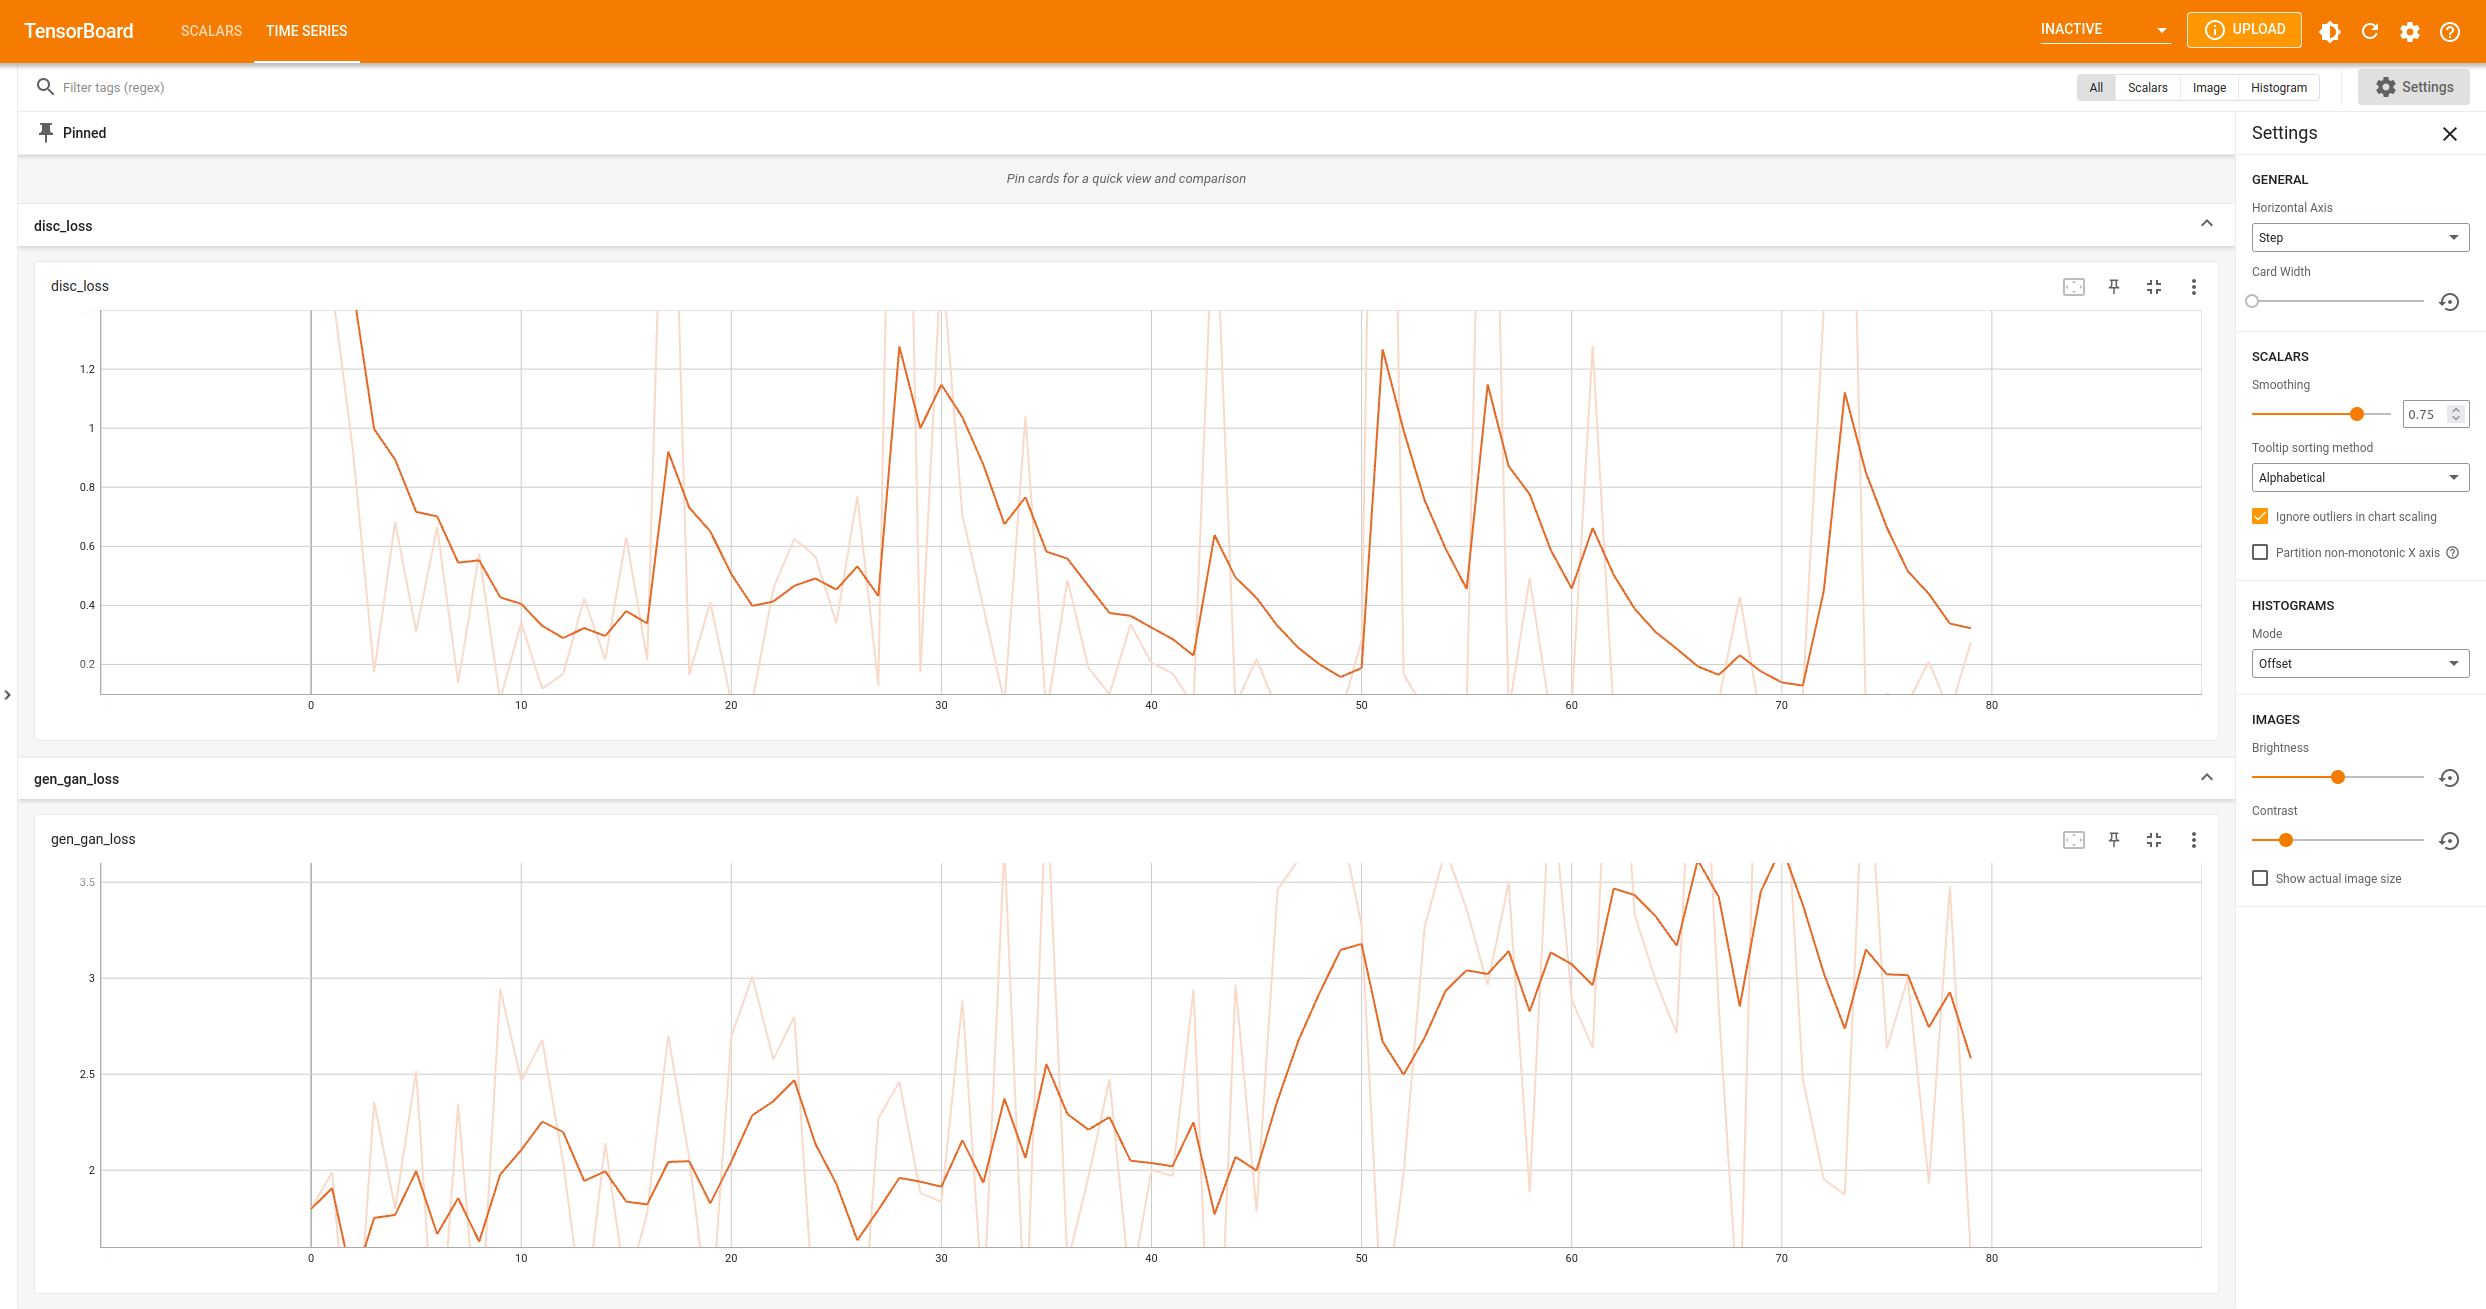
\includegraphics[width=1.0\textwidth]{bilder/tensorboard.png}
	\caption[TensorBoard]{Im TensorBoard können zum Beispiel die Fehlerraten des aktuellen Trainingsdurchlaufs abgelesen oder frühere Trainingsdurchläufe miteinander verglichen werden.}
	\label{fig:unsupervisedexamples}
\end{figure}

In der Funktion \lstinline|fit| wird zuerst ein Bild des Testsets geladen. Das Beispielbild wird verwendet, um durch Aufrufen von \lstinline|generate_images| den aktuellen Trainingserfolg in Form einer Bilddatei im Ausgabeverzeichnis zu speichern. Dieser Vorgang erfolgt nach je 1000 Trainingsschritten.

Über die Trainingsbilder wird wiederholt iteriert und für jedes Trainingsbild \lstinline|train_step| aufgerufen.

Nach je 5000 Trainingsschritten speichert \lstinline|fit| außerdem einen Checkpoint. Dadurch kann einerseits das Training unterbrochen und zu einem späteren Zeitpunkt fortgesetzt werden. Andererseits wird das Modell auf diese Weise persistiert, und es ist später möglich, das künstliche neuronale Netz für seinen eigentlichen Einsatzzweck zu nutzen, ohne es erneut zu trainieren.

Im Ausführungsstrang wird zunächst eine Option des GPU-Speichermanagements gewählt, um die Größe des reservierten Speichers dynamisch anwachsen zu lassen. \cite{zaccone2018tensorflow} Zu Beginn der Experimente hat sich diese Einstellung als vorteilhaft herausgestellt.

Es werden auch einige Parameter wie die Bildgröße und die Größe des Trainingssets und Hyperparameter wie die Batchgröße gesetzt. Das Trainings- und das Testset werden eingelesen, der Generator und die Discriminator erstellt und der Adam-Optimizer initialisiert. Nachdem anschließend das Schreiben der Checkpoints und der Zusammenfassung vorbereitet wurde, erfolgt das Training durch Aufruf von \lstinline|fit|. Im letzten Schritt wird das Modell mit 5 Beispielbildern aus dem Testset aufgerufen.

\chapter{Implementierung}

\section{Entwicklungsumgebung}
\label{sec:env}

\subsection{Ubuntu Linux}
\label{subsec:ubuntu}

\subsection{Python}
\label{subsec:python}

\subsection{Tensorflow}
\label{subsec:tensorflow}

\subsection{CUDA}
\label{subsec:cuda}
Cuda ist eine NVIDIA-proprietäre Hardware- und Software-Architektur.

Es ist das Schema, nach dem NVIDIA-Grafikkarten gebaut wurden, die sowohl traditionelle Grafik-Rendering-Aufgaben als auch allgemeine Aufgaben durchführen können. Zum Programmieren der CUDA GPUs wird die Sprache CUDA C verwendet. CUDA C ist im Wesentlichen die Programmiersprache C mit einer Handvoll Erweiterungen, welche die Programmierung hoch parallelisierter Maschinen wie NVIDIA GPUs ermöglichen. \cite{sanders2010cuda}

Anders als frühere GPU-Generationen, die Rechenressourcen in Vertex- und Pixelshader aufteilten, enthält die CUDA-Architektur eine einheitliche Shader-Pipeline, welche die Zuordnung allgemeiner Berechnungen zu jeder arithmetisch-logischen Einheit (ALU) auf dem Chip durch ein Programm erlaubt. Diese ALUs wurden mit einem Befehlssatz entworfen, der für allgemeine Berechnungen statt für spezielle Grafikberechnungen zugeschnitten ist. Weiterhin wurde den Execution Units auf der GPU freier Lese- und Schreibzugriff auf den Speicher sowie Zugriff auf einen softwaregesteuerten Cache, genannt Shared Memory, gegeben. \cite{sanders2010cuda}

Zusätzlich zu der Sprache für das Schreiben von Code für die GPU stellt NVIDIA einen spezialisierten Hardwaretreiber zur Verfügung, der die hohe Rechenleistung der CUDA-Architektur ausschöpft. Kenntnis der OpenGL- oder DirectX-Programmierschnittstellen ist nicht länger erforderlich. \cite{sanders2010cuda}

\subsection{Image-To-Image-Translation in Python}
Es besteht eine Auswahl an Beispielimplementierungen für Image-To-Image-Translation. Das Original-Paper verweist auf ein GitHub-Repository, das eine Lua-Implementierung zur Verfügung stellt. Wegen der besseren Eignung für Experimente auf einem lokalen Rechner durch CUDA-Unterstützung mit Tensorflow wird in dieser Arbeit Python verwendet.

Die verwendete Beispielimplementierung ist zum Zeitpunkt der Erstellung dieses Dokumentes unter https://github.com/tensorflow/docs/blob/master/site/en/tutorials/generative/pix2pix.ipynb zu finden. Eine an die aktuelle Version von Tensorflow und die Anforderungen dieser Arbeit angepasste Version befindet sich im Anhang.

Die wichtigste Änderung ist das selbst erstellte Dataset, das statt der im Beispiel verwendeten Gebäudefassaden geladen wird. Es wurden Ausgaben entfernt, wegen derer die Ausführung des Skriptes unterbrochen wurde. Dabei wurden Bildinformationen und Beispielbilder nach dem Laden des Datasets, dem Aufteilen in Eingabebild und Ground Truth, der Erzeugung von Bildrauschen, Down- und Upsampling sowie den ersten Trainingsdurchläufen ausgegeben, die während des Trainings der Skizzen- und Renderbilder nicht betrachtet werden mussten. Außerdem wurden bei jedem Training Diagramme des Generators und des Discriminators erzeugt.


\chapter{Experimente und Resultate}
\label{ch:conduct}

\section{Vorbereitung der Eingabedaten}
\label{sec:preparation}
Die Trainingsdaten liegen für das ``Quick, Draw!''-Dataset im NDJSON-Format und als Blender-Dateien beziehungsweise
Wavefront OBJ-Dateien vor. Die effizienteste Möglichkeit, die Skizzen und 3D-Modelle für die Verarbeitung in einem CNN vorzubereiten, ist das Rendern und  Speichern als Bilddateien. Als Dateiformat kommen JPEG oder PNG infrage. Beide Formate können leicht als Trainingsset mit Tensorflow geladen werden.

NDJSON steht für Newline Delimited JavaScript Object Notation. In einer solchen Datei sind also zeilenweise JSON-Objekte gespeichert. Für jede Zeichnung sind Angaben zu Motiv, Ort und Zeit enthalten. Außerdem ist angegeben, ob die künstliche Intelligenz des Minispiels das Motiv in der Zeichnung korrekt klassifiziert, also erkannt hat. Jede Zeichnung hat weiterhin eine eindeutige ID.

Der relevanteste Teil ist die ``Drawings''-Eigenschaft der JSON-Objekte, ein mehrdimensionales Array mit Bildkoordinaten. Es enthält mindestens X-Koordinaten und Y-Koordinaten in jeweils einem Array im ``Drawings''-Array. Indem Linien zwischen den Bildkoordinaten in der Reihenfolge der Arrayelemente in ein Bild gezeichnet und in einer Bilddatei gespeichert werden, können die Zeichnungen in beliebigen Bilddateiformaten gespeichert werden. Für diese Arbeit wurde die Konvertierung ebenfalls in Python realisiert.

Bei der Verarbeitung in einem Convolutional Neural Network spielt die Bildgröße
in Bezug auf die Verarbeitungszeit eine wichtige Rolle. Bildformate der Größe 256x256 oder kleiner sind üblich und gut geeignet. Für ein GAN ist es zwar nicht erforderlich, aber sinnvoll, für Ein- und Ausgabedaten dieselben Dimensionen festzulegen. Bei der Bildgenerierung aus Skizzen unterscheiden sich Ein- und Ausgabdedaten natürlich bei die Farbtiefe. Während die Skizzen Graustufenbilder sind, besitzen die generierten Bilder drei Farbkanäle (RGB).

Sowohl während der Entwicklung als auch zur Laufzeit kann es vorteilhaft sein, Farbwerte statt auf der oft verwendeten Skala von $0$ bis $255$ als Fließkommazahlen im Bereich $0,0$ bis $1,0$ darzustellen. Auch für die Ausgaben der einzelnen Schichten eines künstlichen neuronalen Netzes kann diese Normalisierung durchgeführt werden (TODO: BatchNorm).

Ein ebenso wichtiger wie aufwendiger Vorgang ist die Klassifizierung der Trainingsdaten, also die Zuweisung von Eingaben zu den erlernbaren Ergebnissen. Aufgrund der selbst erstellten Ausgabebilder existieren für diesen Zweck keine vorgefertigten Datasets. Die Sortierung und Zuweisung erfolgt deshalb manuell.


\section{Anwendung herkömmlicher Shader}
\label{sec:shader}
Shader definieren die Interaktion des Lichts mit der Oberfläche des Objekts. Dabei können Shader aus einem oder mehreren BSDFs (Bidirectional Scattering Distribution Function) bestehen, die wiederum von Mix-und Add-Shadern in der Zusammensetzung gemischt werden. \cite{wartmann2014blender}

In der Computergrafik wird die Darstellung der Oberfläche eines Objekts durch die drei Faktoren Material, Textur und Ausleuchtung bestimmt. Material ist die Grundfarbe der Oberfläche. Textur sind die physischen Charakteristiken der Oberfläche, und Ausleuchtung ist die Hintergrundbeleuchtung oder Licht, welches von Lichtern (Lampen) emittiert wird. \cite{blain2020blender}

In der Computergrafik ist ein Material die Farbe eines Objektes. Es legt fest, wie das sichtbare Spektrum des Lichts von der Oberfläche des Objekts reflektiert wird. Ein Material legt außerdem fest, ob die Oberfläche matt oder metallisch erscheint. \cite{blain2020blender}

Material (Farbe) kann entsprechend der drei Farbschemas RGB, HSV oder Hex dargestellt werden. Wie die Farbe in jedem Schema erscheint ist auch von einem Alpha-Wert, welcher für die Menge der Transparenz steht, abhängig. \cite{blain2020blender}

Texturen definieren das physische Erscheinungsbild einer Oberfläche, also etwa wie glatt oder uneben diese erscheint, oder ihre Struktur, welche die visuelle Wahrnehumg der physischen Beschaffenheit des Objekts definiert. Diese Definition bestimmt, woraus die Oberfläche besteht, wie Holz, Ziegelsteine, Wasser und so weiter. \cite{blain2020blender}

Texturen werden durch Algorithmen generiert, wie sie in Blender integriert sind (prozedurale Texturen) oder aus Bilddateien (Bildtexturen). \cite{blain2020blender}

Die Qualität eines Bildes hängts direkt von der Effektivität des Shading-Algorithmus ab, der wiederum von der Modellierungsmethode des Objektes abhängt. Zwei wesentliche Methoden der Objektbeschreibung werden häufig verwendet, nämlich Oberflächendefinition mittels mathematischer Gleichungen und Oberflächenapproximation durch Mosaike aus polygonalen Flächen. \cite{phong1975shading}

Polygonobjekte sind anfangs immer ungeglättet, das heißt, dass beim Rendern oder in der schattierten Ansicht zunächst immer die einzelnen Flächen zu sehen sind, aus denen sich das Objekt zusammensetzt. Eine mögliche, wenn auch in Sachen Renderzeit und Speicherverbrauch ungünstige Methode wäre, einfach das Objekt so weit in kleinere Flächen zu unterteilen, dass beim Rendern eine Fläche pro Pixel gerendert wird. In der praktischen Arbeit verwendet man deshalb einen Trick, bei dem die Übergänge zwischen den einzelnen Flächen ``glattgerechnet'' werden. Übliche Verfahren hier sind das Gouraud oder Phong Shading. \cite{wartmann2014blender}

\section{Hyperparameter}
\label{sec:hyperparams}
Die Pix2Pix-Referenzimplementierung ist bereits für die Übersetzung von Skizzen in Fotos eingestellt. Für das Training waren anfangs mehrere Tausend Epochs, also Trainingsdurchläufe, erfoderlich, um zufriedenstellende Ergebnisse zu sehen. TODO: Diese Zahl konnte durch ... verringert werden.

Die Eingabebilder sind 256x256 Pixel groß und besitzen einen Farbkanal für Graustufen. Sie werden am Anfang des Trainingsprozesses durch sogenanntes Jittering augmentiert. Dabei werden die Bilder zuerst auf 286x268 Pixel vergrößert und anschließend auf einen zufälligen 256x256 Pixel großer Ausschnitt wieder verkleinert. Diese  Pixelgrößen können im Experiment geändert werden.

Der Adam Optimierer \cite{kingma2017adam} erhält für die Learning-Rate den Wert $0,0002$. Das Momentum ist auf $0,9$ voreingestellt. Diese beiden Werte beinflussen die Lerngeschwindigkeit und sind in begrenztem Maße anpassbar.

\section{Performancebeobachtungen}
\label{sec:performance}


\chapter{Diskussion}
\label{sec:conclusion}


%weitere Kapitel hier einfügen

%\cleardoublepage
%\input{03_neues_kapitel}

%Literatur
\cleardoublepage
\printbibliography[heading=bibintoc]

%Bildnachweise
\cleardoublepage
\chapter*{Bildnachweis}
\addcontentsline{toc}{chapter}{Bildnachweis}

% \autoref{fig:trichter}: The Metropolitan Museum of Art,\\
% https://www.metmuseum.org/art/collection/search/202901, (CC0 1.0)

\autoref{fig:tensorboard}: {TensorFlow}: Large-Scale Machine Learning on Heterogeneous Systems,\\
https://www.tensorflow.org/, (CC BY 4.0 / Apache License 2.0) \\

\noindent
\autoref{fig:blender}: Blender Foundation,\\
https://www.blender.org/, (GNU GPLv3)

\noindent
\autoref{fig:pix2pixprogress3}: {TensorFlow}: Large-Scale Machine Learning on Heterogeneous Systems,\\
https://www.tensorflow.org/, (CC BY 4.0 / Apache License 2.0) \\

\noindent
\autoref{fig:pix2pixprogress4}: {TensorFlow}: Large-Scale Machine Learning on Heterogeneous Systems,\\
https://www.tensorflow.org/, (CC BY 4.0 / Apache License 2.0) \\

\noindent
TensorFlow, the TensorFlow logo and any related marks are trademarks of Google Inc.


%Abbildungsverzeichnis
\cleardoublepage
\addcontentsline{toc}{chapter}{\listfigurename}
\listoffigures

%Tabellenverzeichnis
\cleardoublepage
\addcontentsline{toc}{chapter}{\listtablename}
\listoftables

%Anhang
\cleardoublepage
\appendix
\addtocontents{toc}{\protect\newpage}
\part*{Anhang}
\addcontentsline{toc}{chapter}{Anhang}

\chapter{Quelltexte}
\label{ch:a_sim}

\section{Image-To-Image-Translation main.py}
\label{pix2pixpy}

\begin{lstlisting}
import tensorflow as tf

import os
import time
import datetime

from matplotlib import pyplot as plt
from IPython import display

from tensorflow.compat.v1 import ConfigProto
from tensorflow.compat.v1 import InteractiveSession


def load(image_file):
    # Read and decode an image file to a uint8 tensor
    image = tf.io.read_file(image_file)
    image = tf.image.decode_jpeg(image)

    # Split each image tensor into two tensors:
    w = tf.shape(image)[1]
    w = w // 2
    input_image = image[:, :w, :]
    real_image = image[:, w:, :]

    # Convert both images to float32 tensors
    input_image = tf.cast(input_image, tf.float32)
    real_image = tf.cast(real_image, tf.float32)

    return input_image, real_image


def resize(input_image, real_image, height, width):
    input_image = tf.image.resize(
      input_image, [height, width], method=tf.image.ResizeMethod.NEAREST_NEIGHBOR)
    real_image = tf.image.resize(
      real_image, [height, width], method=tf.image.ResizeMethod.NEAREST_NEIGHBOR)

    return input_image, real_image


def random_crop(input_image, real_image):
    stacked_image = tf.stack([input_image, real_image], axis=0)
    cropped_image = tf.image.random_crop(
      stacked_image, size=[2, IMG_HEIGHT, IMG_WIDTH, 3]
    )

    return cropped_image[0], cropped_image[1]
\end{lstlisting}
\pagebreak
\begin{lstlisting}
# Normalizing the images to [-1, 1]
def normalize(input_image, real_image):
    input_image = (input_image / 127.5) - 1
    real_image = (real_image / 127.5) - 1

    return input_image, real_image


@tf.function()
def random_jitter(input_image, real_image):
    # Resizing to 286x286
    input_image, real_image = resize(input_image, real_image, 286, 286)

    # Random cropping back to 256x256
    input_image, real_image = random_crop(input_image, real_image)

    if tf.random.uniform(()) > 0.5:
        # Random mirroring
        input_image = tf.image.flip_left_right(input_image)
        real_image = tf.image.flip_left_right(real_image)

    return input_image, real_image


def load_image_train(image_file):
    input_image, real_image = load(image_file)
    input_image, real_image = random_jitter(input_image, real_image)
    input_image, real_image = normalize(input_image, real_image)

    return input_image, real_image


def load_image_test(image_file):
    input_image, real_image = load(image_file)
    input_image, real_image = resize(
      input_image, real_image, IMG_HEIGHT, IMG_WIDTH
    )
    input_image, real_image = normalize(input_image, real_image)

    return input_image, real_image


def downsample(filters, size, apply_batchnorm=True):
    initializer = tf.random_normal_initializer(0., 0.02)

    result = tf.keras.Sequential()
    result.add(
      tf.keras.layers.Conv2D(
        filters,
        size,
        strides=2,
        padding='same',
        kernel_initializer=initializer,
        use_bias=False
      )
    )

    if apply_batchnorm:
        result.add(tf.keras.layers.BatchNormalization())

    result.add(tf.keras.layers.LeakyReLU())

    return result

\end{lstlisting}
\pagebreak
\begin{lstlisting}
def upsample(filters, size, apply_dropout=False):
    initializer = tf.random_normal_initializer(0., 0.02)

    result = tf.keras.Sequential()
    result.add(
        tf.keras.layers.Conv2DTranspose(
            filters, size, strides=2,
            padding='same',
            kernel_initializer=initializer,
            use_bias=False
        )
    )

    result.add(tf.keras.layers.BatchNormalization())

    if apply_dropout:
        result.add(tf.keras.layers.Dropout(0.5))

    result.add(tf.keras.layers.ReLU())

    return result


def build_generator():
    inputs = tf.keras.layers.Input(shape=[256, 256, 3])

    down_stack = [
        downsample(64, 4, apply_batchnorm=False),  # (batch_size, 128, 128, 64)
        downsample(128, 4),  # (batch_size, 64, 64, 128)
        downsample(256, 4),  # (batch_size, 32, 32, 256)
        downsample(512, 4),  # (batch_size, 16, 16, 512)
        downsample(512, 4),  # (batch_size, 8, 8, 512)
        downsample(512, 4),  # (batch_size, 4, 4, 512)
        downsample(512, 4),  # (batch_size, 2, 2, 512)
        downsample(512, 4),  # (batch_size, 1, 1, 512)
    ]

    up_stack = [
        upsample(512, 4, apply_dropout=True),  # (batch_size, 2, 2, 1024)
        upsample(512, 4, apply_dropout=True),  # (batch_size, 4, 4, 1024)
        upsample(512, 4, apply_dropout=True),  # (batch_size, 8, 8, 1024)
        upsample(512, 4),  # (batch_size, 16, 16, 1024)
        upsample(256, 4),  # (batch_size, 32, 32, 512)
        upsample(128, 4),  # (batch_size, 64, 64, 256)
        upsample(64, 4),  # (batch_size, 128, 128, 128)
    ]

    initializer = tf.random_normal_initializer(0., 0.02)
    last = tf.keras.layers.Conv2DTranspose(
        OUTPUT_CHANNELS,
        4,
        strides=2,
        padding='same',
        kernel_initializer=initializer,
        activation='tanh'
    )  # (batch_size, 256, 256, 3)

    x = inputs

    # Downsampling through the model
    skips = []
    for down in down_stack:
        x = down(x)
        skips.append(x)

    skips = reversed(skips[:-1])

\end{lstlisting}
\pagebreak
\begin{lstlisting}
    # Upsampling and establishing the skip connections
    for up, skip in zip(up_stack, skips):
        x = up(x)
        x = tf.keras.layers.Concatenate()([x, skip])

    x = last(x)
    return tf.keras.Model(inputs=inputs, outputs=x)


def generator_loss(disc_generated_output, gen_output, target):
    gan_loss = loss_object(tf.ones_like(disc_generated_output), disc_generated_output)

    # Mean absolute error
    l1_loss = tf.reduce_mean(tf.abs(target - gen_output))

    total_gen_loss = gan_loss + (LAMBDA * l1_loss)

    return total_gen_loss, gan_loss, l1_loss


def build_discriminator():
    initializer = tf.random_normal_initializer(0., 0.02)

    inp = tf.keras.layers.Input(shape=[256, 256, 3], name='input_image')
    tar = tf.keras.layers.Input(shape=[256, 256, 3], name='target_image')

    x = tf.keras.layers.concatenate([inp, tar])  # (batch_size, 256, 256, channels*2)

    down1 = downsample(64, 4, False)(x)  # (batch_size, 128, 128, 64)
    down2 = downsample(128, 4)(down1)  # (batch_size, 64, 64, 128)
    down3 = downsample(256, 4)(down2)  # (batch_size, 32, 32, 256)

    zero_pad1 = tf.keras.layers.ZeroPadding2D()(down3)  # (batch_size, 34, 34, 256)
    conv = tf.keras.layers.Conv2D(
        512,
        4,
        strides=1,
        kernel_initializer=initializer,
        use_bias=False
    )(zero_pad1)  # (batch_size, 31, 31, 512)

    batchnorm1 = tf.keras.layers.BatchNormalization()(conv)

    leaky_relu = tf.keras.layers.LeakyReLU()(batchnorm1)

    zero_pad2 = tf.keras.layers.ZeroPadding2D()(leaky_relu)  # (batch_size, 33, 33, 512)

    last = tf.keras.layers.Conv2D(
        1, 4, strides=1, kernel_initializer=initializer
    )(zero_pad2)  # (batch_size, 30, 30, 1)

    return tf.keras.Model(inputs=[inp, tar], outputs=last)


def discriminator_loss(disc_real_output, disc_generated_output):
    real_loss = loss_object(tf.ones_like(disc_real_output), disc_real_output)

    generated_loss = loss_object(tf.zeros_like(disc_generated_output), disc_generated_output)

    total_disc_loss = real_loss + generated_loss

    return total_disc_loss


def generate_images(model, test_input, tar, image_index):
    prediction = model(test_input, training=True)
    plt.figure(figsize=(15, 15))

    display_list = [test_input[0], tar[0], prediction[0]]
    title = ['Input Image', 'Ground Truth', 'Predicted Image']

    for i in range(3):
        plt.subplot(1, 3, i + 1)
        plt.title(title[i])
        # Getting the pixel values in the [0, 1] range to plot.
        plt.imshow(display_list[i] * 0.5 + 0.5)
        plt.axis('off')

    plt.savefig('results/' + str(image_index) + '.jpg')


@tf.function
def train_step(input_image, target, step):
    with tf.GradientTape() as gen_tape, tf.GradientTape() as disc_tape:
        gen_output = generator(input_image, training=True)

        disc_real_output = discriminator([input_image, target], training=True)
        disc_generated_output = discriminator([input_image, gen_output], training=True)

        gen_total_loss, gen_gan_loss, gen_l1_loss =
            generator_loss(disc_generated_output, gen_output, target)
        disc_loss = discriminator_loss(disc_real_output, disc_generated_output)

    generator_gradients = gen_tape.gradient(
        gen_total_loss, generator.trainable_variables
    )
    discriminator_gradients = disc_tape.gradient(
        disc_loss, discriminator.trainable_variables
    )

    generator_optimizer.apply_gradients(
        zip(generator_gradients, generator.trainable_variables)
    )
    discriminator_optimizer.apply_gradients(
        zip(discriminator_gradients, discriminator.trainable_variables)
    )

    with summary_writer.as_default():
        tf.summary.scalar('gen_total_loss', gen_total_loss, step=step // 1000)
        tf.summary.scalar('gen_gan_loss', gen_gan_loss, step=step // 1000)
        tf.summary.scalar('gen_l1_loss', gen_l1_loss, step=step // 1000)
        tf.summary.scalar('disc_loss', disc_loss, step=step // 1000)


def fit(train_ds, test_ds, steps):
    example_input, example_target = next(iter(test_ds.take(1)))
    start = time.time()

    for step, (input_image, target) in train_ds.repeat().take(steps).enumerate():
        if step % 1000 == 0:
            display.clear_output(wait=True)

            if step != 0:
                print(f'Time taken for 1000 steps: {time.time() - start:.2f} sec\n')

            start = time.time()

            generate_images(generator, example_input, example_target, step.numpy() // 1000)
            print(f"Step: {step // 1000}k")

        train_step(input_image, target, step)

        # Training step
        if (step + 1) % 10 == 0:
            print('.', end='', flush=True)

        # Save (checkpoint) the model every 5k steps
        if (step + 1) % 5000 == 0:
            checkpoint.save(file_prefix=checkpoint_prefix)


if __name__ == '__main__':
    config = ConfigProto()
    config.gpu_options.allow_growth = True
    session = InteractiveSession(config=config)

    # Adjust this value to the number of training images
    BUFFER_SIZE = 400

    # The batch size of 1 produced better results
    # for the U-Net in the original pix2pix experiment
    BATCH_SIZE = 1

    # Each image is 256x256 in size
    IMG_WIDTH = 256
    IMG_HEIGHT = 256

    PATH = '../PIX2PIX/images/combined/candles/'
    train_dataset = tf.data.Dataset.list_files(PATH + 'train/*.png')
    train_dataset = train_dataset.map(
      load_image_train, num_parallel_calls=tf.data.AUTOTUNE
    )
    train_dataset = train_dataset.shuffle(BUFFER_SIZE)
    train_dataset = train_dataset.batch(BATCH_SIZE)

    try:
        test_dataset = tf.data.Dataset.list_files(str(PATH + 'test/*.png'))
    except tf.errors.InvalidArgumentError:
        test_dataset = tf.data.Dataset.list_files(str(PATH + 'val/*.png'))
    test_dataset = test_dataset.map(load_image_test)
    test_dataset = test_dataset.batch(BATCH_SIZE)

    OUTPUT_CHANNELS = 3

    generator = build_generator()

    LAMBDA = 100

    loss_object = tf.keras.losses.BinaryCrossentropy(from_logits=True)

    discriminator = build_discriminator()

    generator_optimizer = tf.keras.optimizers.Adam(2e-4, beta_1=0.5)
    discriminator_optimizer = tf.keras.optimizers.Adam(2e-4, beta_1=0.5)

    checkpoint_dir = './training_checkpoints'
    checkpoint_prefix = os.path.join(checkpoint_dir, "ckpt")
    checkpoint = tf.train.Checkpoint(
        generator_optimizer=generator_optimizer,
        discriminator_optimizer=discriminator_optimizer,
        generator=generator,
        discriminator=discriminator
    )

    log_dir = "logs/"

    summary_writer = tf.summary.create_file_writer(
        log_dir + "fit/" + datetime.datetime.now().strftime("%Y%m%d-%H%M%S")
    )

    fit(train_dataset, test_dataset, steps=40000)

\end{lstlisting}
\pagebreak
\begin{lstlisting}
    # Restoring the latest checkpoint in checkpoint_dir
    checkpoint.restore(tf.train.latest_checkpoint(checkpoint_dir))

    # Run the trained model on a few examples from the test set
    index = 1000
    for inp, tar in test_dataset.take(5):
        generate_images(generator, inp, tar, index)
        index = index + 1

\end{lstlisting}
\vfill

\pagebreak

\section{Python-Script zur Generierung von JPEG-Bilddateien aus NDJSON-Informationen}
\label{ndjsonpy}

\begin{lstlisting}
import os
from functools import reduce
import tensorflow as tf
import json
from PIL import Image, ImageDraw

MAX_JPGS = 5000

dataset = tf.data.TextLineDataset(['../full_simplified_car.ndjson'])

for index, line in enumerate(dataset):
    if index % 1000 == 0:
        print(f'{index} of {MAX_JPGS}')
    jsonLine = json.loads(line.numpy())
    drawing = jsonLine['drawing']

    im = Image.new('RGB', (256, 256), (255, 255, 255))
    draw = ImageDraw.Draw(im)

    # normalise coords to center the drawing
    x_coords = reduce(lambda a, b: a + b, [stroke[0] for stroke in drawing])
    displacement_x = int((256 - min(x_coords) - max(x_coords)) / 2)
    y_coords = reduce(lambda a, b: a + b, [stroke[1] for stroke in drawing])
    displacement_y = int((256 - min(y_coords) - max(y_coords)) / 2)

    for stroke in drawing:
        draw.line(list(zip(
          [x + displacement_x for x in stroke[0]],
          [y + displacement_y for y in stroke[1]]
        )), fill=0)

    im.save(os.path.join('cars', str(index) + '.jpg'), 'JPEG')

    with open(os.path.join('json', str(index) + '.json'), 'w') as file:
        file.write(json.dumps(drawing))

    if index == MAX_JPGS:
        break
\end{lstlisting}
\vfill

\pagebreak

\section{Blender-Python-Script zur Generierung von Tischen}
\label{blenderpy}

\begin{lstlisting}
import bpy
import math
import random

obj_filepath = '/home/sberger/blender/tables/obj/random_table{}.obj'
render_filepath = '/home/sberger/blender/tables/rendered/random_table{}_render{}.jpg'

for tableIndex in range(0, 50):
    # add table top
    tableWidth = random.random() * 8 + 6
    tableHeight = random.random() * .5 + .1
    tableDepth = random.random() * 4 + 4
    legLength = random.random() * 4 + 1
    bpy.ops.mesh.primitive_cube_add(
      size=1, enter_editmode=False, location=(0, tableHeight / 2 + legLength, 0)
    )
    bpy.context.object.name = 'Table'
    bpy.ops.transform.resize(
      value=(tableWidth, tableHeight, tableDepth),
      orient_type='GLOBAL',
      orient_matrix=((1, 0, 0), (0, 1, 0), (0, 0, 1)),
      orient_matrix_type='GLOBAL',
      constraint_axis=(False, True, False),
      mirror=True, use_proportional_edit=False,
      proportional_edit_falloff='SMOOTH',
      proportional_size=1,
      use_proportional_connected=False,
      use_proportional_projected=False
    )
    bpy.context.active_object.data.materials.append(bpy.data.materials.get("Wood"))

    # add table legs
    legWidth = random.random() * .5 + .1
    legDisplacement = random.random() * 1 + legWidth / 2
    legDisplacementX = tableWidth / 2 - legDisplacement
    legDisplacementZ = tableDepth / 2 - legDisplacement

    for legIndex, coords in enumerate([
      [legDisplacementX, legDisplacementZ],
      [-legDisplacementX, legDisplacementZ],
      [legDisplacementX, -legDisplacementZ],
      [-legDisplacementX, -legDisplacementZ]
    ]):
        bpy.ops.mesh.primitive_cube_add(
          size=1, enter_editmode=False, location=(coords[0], legLength / 2, coords[1])
        )
        bpy.context.object.name = 'TableLeg' + str(legIndex)
        bpy.ops.transform.resize(
          value=(legWidth, legLength, legWidth),
          orient_type='GLOBAL',
          orient_matrix=((1, 0, 0), (0, 1, 0), (0, 0, 1)),
          orient_matrix_type='GLOBAL',
          constraint_axis=(False, True, False),
          mirror=True,
          use_proportional_edit=False,
          proportional_edit_falloff='SMOOTH',
          proportional_size=1,
          use_proportional_connected=False,
          use_proportional_projected=False
        )
        bpy.context.active_object.data.materials.append(bpy.data.materials.get("Wood"))

    # export to wavefront obj format
    bpy.ops.export_scene.obj(filepath = obj_filepath.format(tableIndex))

    # rotate and render
    bpy.ops.object.select_all(action='DESELECT')
    bpy.data.objects['Table'].select_set(True)
    for legIndex in range(0, 4):
        bpy.data.objects['TableLeg' + str(legIndex)].select_set(True)
    bpy.ops.object.transform_apply(location=False, rotation=True, scale=False)
    for renderIndex in range(0, 5):
        # rotate table
        bpy.ops.transform.rotate(
          value=math.pi / 5,
          orient_axis='Y',
          orient_type='GLOBAL',
          orient_matrix=((1, 0, 0), (0, 1, 0), (0, 0, 1)),
          orient_matrix_type='GLOBAL',
          constraint_axis=(False, True, False),
          mirror=True,
          use_proportional_edit=False,
          proportional_edit_falloff='SMOOTH',
          proportional_size=1,
          use_proportional_connected=False,
          use_proportional_projected=False
        )

        # render
        bpy.context.scene.render.filepath = render_filepath.format(tableIndex, renderIndex)
        bpy.ops.render.render(write_still = True)

    #delete objects
    bpy.ops.object.delete(use_global=False)
\end{lstlisting}


\end{document}
